


\documentclass[5pt]{article}

\usepackage{sectsty}
\usepackage{graphicx}
\usepackage{lipsum} % for generating dummy text
\usepackage[margin=1in]{geometry}
\usepackage{setspace}
\usepackage{array}
\usepackage{cellspace}
\usepackage{tabularx}
\usepackage[table]{xcolor}
\usepackage{tabularray}
\usepackage{pgfplots}
\usepackage{caption}
\DeclareCaptionLabelFormat{blank}{}

\usepackage{eurosym}



\usepackage{hyperref}
\usepackage{scrextend}
\graphicspath{ {../assets} }


% package and setup for tables
\usepackage{float}
\usepackage[table]{xcolor}
\renewcommand{\arraystretch}{1.5}
\arrayrulecolor{black}


% Margins
\topmargin=-0.45in
\evensidemargin=0in
\oddsidemargin=0in
\textwidth=6.5in
\textheight=9.0in
\headsep=0.25in

\setlength{\parindent}{0pt}

\title{Piano di Qualifica}
\author{Jackpot Coding}
\renewcommand*\contentsname{Indice}
\date{\today}

%STARTOF THE DOCUMENT
\begin{document}
	
	%-------------------------
	
	% Reduce top margin only on the first page
	\newgeometry{top=0.5in}
	
	%UNIPD LOGO
	\vspace{8pt}
	
\includegraphics[scale=0.2]{UNIPDFull.png}
	%END UNIPD LOGO
	
	\vspace{30pt}
	
	%COURSE INFO
	\begin{minipage}[t]{0.48\textwidth}
		%COURSE TITLE
		\begin{flushleft}
			Informatica\\
			\vspace{5pt}
			\textbf{\LARGE Ingegneria del Software}\\
			Anno Accademico: 2023/2024
		\end{flushleft}
		%END COURSE TITLE
	\end{minipage}
	%END COURSE INFO
	
	
	\vspace{5px}
	
	
	%BLACK LINE
	\rule{\textwidth}{5pt}
	
	%JACKPOT CODING INFO
	\begin{minipage}[t]{0.50\textwidth}
		%LOGO JACKPOT CODING
		\begin{flushleft}
			\hspace{10pt}
			
\includegraphics[scale=0.65]{jackpot-logo.png} 
		\end{flushleft}
	\end{minipage}
	\hspace{-60pt} % This adds horizontal space between the minipages
	\begin{flushright}
		\begin{minipage}[t]{0.50\textwidth}
			%INFO JACKPOT CODING
			\begin{flushright}
				Gruppo: {\Large Jackpot Coding}\\
				Email: \href{mailto:jackpotcoding@gmail.com}{jackpotcoding@gmail.com}
			\end{flushright}
		\end{minipage}
	\end{flushright}
	%END JACKPOT CODING INFO
	
	\vspace{24pt}
	
	%TITLE
	\begin{center}
		\textbf{\LARGE PIANO DI QUALIFICA}
	\end{center}
	%END TITLE
	
	\vspace{13pt}
	
	\begin{flushleft}
		\begin{spacing}{1.5}
			REDATTORI: G. Moretto, R. Simionato, M. Gobbo\\%INSERT HERE THE NAMES
			VERIFICATORI: M. Gobbo, M. Favaretto, G. Moretto, R. Simionato\\
			\vspace{7pt}
			DESTINATARI: Prof. T. Vardanega, Prof. R. Cardin\\%INSERT HERE THE NAMES
		\end{spacing}
	\end{flushleft}
	
	\begin{flushright}
		\begin{spacing}{1}
			USO: ESTERNO\\
			VERSIONE: 2.0.0\\
		\end{spacing}
	\end{flushright}
	
	
	% Restore original margins from the second page onwards
	\restoregeometry
	
	\pagebreak
	
	\textbf{\Large Registro delle modifiche}
	\begin{table}[H]
		\centering
		\rowcolors{2}{black!15}{}
		\resizebox{\linewidth}{!}{
			\begin{tabular}{|c|c|c|c|c|}
				\rowcolor{teal!50}
				\hline
				\textbf{Versione} & \textbf{Data} & \textbf{Autore} & \textbf{Verificatore} & \textbf{Modifica} \\
                                \hline
                                v.2.0.0 & 12/05/2024 & - & M. Gobbo & Approvazione alla 2.0.0\\
				\hline
				v.1.0.9 & 09/05/2024 & G.Moretto & M. Gobbo & Aggiornamento grafici con dati finali \\
				\hline
				v.1.0.7 & 07/05/2024 & G.Moretto & M.Gobbo & Aggiunti test di integrazione e regressione \\
				\hline
				v.1.0.6 & 07/05/2024 & G.Moretto & M.Gobbo & Termini glossario, grafico quality metrics satisfied e requisiti obbligatori \\
				\hline
				v.1.0.5 & 28/04/2024 & G.Moretto & M. Gobbo & Aggiunta spiegazioni su grafici, elenco immagini e tabelle\\
				\hline
				v.1.0.4 & 27/04/2024 & G.Moretto & M. Gobbo &Tolti failure density, test da Integrazione a sistema, grafici MPC-PTP,PMC-BV,MPD-CS,MPC-CD,MPC-AC, MPC-ETC e MPC-EAC \\
				\hline
				v.1.0.3 & 25/04/2024 & R. Simionato & G. Moretto & Aggiunti riferimenti al Glossario per le metriche \\
				\hline
				v.1.0.2 & 03/04/2024 & E. Gallo & M.Gobbo & Aggiunti riferimenti normativi ed informativi \\
				\hline
				v.1.0.1 & 26/03/2024 & E. Gallo & M. Gobbo & Aggiunti Elenco delle immagini ed Elenco delle tabelle \\
				\hline
				v.1.0.0 & 23/03/2024 & - & M. Favaretto & Verifica documento \\
				\hline
				v.0.1.12 & 22/03/2024 & G. Moretto & M. Favaretto & Aggiunta indicazione per dati mancanti prima della PB\textsuperscript{G} \\
				\hline
				v.0.1.12 & 22/03/2024 & G. Moretto & M. Gobbo & Aggiunta indicazione per dati mancanti prima della PB\textsuperscript{G} \\
				\hline
				v.0.1.11 & 22/03/2024 & G. Moretto & M. Gobbo & Aggiornamento grafici MPC-CV, MPC-AC e MPC-ETC, MPC-SV \\
				\hline
				v.0.1.10 & 21/03/2024 & G. Moretto & M. Gobbo & Aggiunti grafici MPC-CV, MPC-AC e MPC-ETC, MPC-SV \\
				\hline
				v.0.1.9 & 21/03/2024 & R. Simionato & G. Moretto & Aggiunte strutture grafici MPC-CV, MPC-AC e MPC-ETC \\
				\hline
				v.0.1.8 & 20/03/2024 & R. Simionato & G. Moretto & \shortstack{Aggiunti grafici MPC-RSI e MPD-CO\\Aggiunte sottosezioni per altri grafici} \\
				\hline
				v.0.1.7 & 19/03/2024 & G. Moretto & M. Gobbo & Aggiunta grafico MPD-I \\
				\hline
				v.0.1.6 & 19/03/2024 & G. Moretto & M. Gobbo & Aggiunta grafici MPC-SV e MPC-NCR \\
				\hline
				v.0.1.5 & 18/03/2024 & G. Moretto & M. Gobbo & Verifica termini di glossario \\
				\hline
				v.0.1.4 & 18/03/2024 & R. Simionato & G. Moretto & Stesura sezioni 2.1.2, 2.2, 2.3 \\
				\hline
				v.0.1.3 & 17/03/2024 & M. Gobbo & G. Moretto & Aggiunta Sezione 3-Qualità di Prodotto \\
				\hline
				v.0.1.2 & 17/03/2024 & R. Simionato & G. Moretto & Aggiunta struttura Sezione 3-Qualità di Prodotto \\
				\hline
				v.0.1.1 & 16/03/2024 & R. Simionato & G. Moretto & \shortstack{Prima stesura sezione Qualità di Processo\\e inserimento tabelle} \\
				\hline
				v.0.1.0 & 16/03/2024 & - & R. Simionato & Verifica Documento \\
				\hline
				v.0.0.3 & 14/03/2024 & G. Moretto & R. Simionato & Aggiunta sezione Valutazione attività di verifica \\
				\hline
				v.0.0.2 & 13/02/2024 & G. Moretto & R. Simionato  &  Aggiunte descrizioni test\\
				\hline
				v.0.0.1 & 03/02/2024 & G. Moretto & R. Simionato  & Creata struttura del documento \\
				\hline
	   		\end{tabular}
		}
	 	\label{tab:conference}
    \end{table}

	\pagebreak
	\tableofcontents
	\pagebreak

	\textbf{\Large Elenco delle immagini} \\
	\makeatletter
	\@starttoc{lof}% Print List of Figures
	\makeatother
	
	\pagebreak
	\textbf{\Large Elenco delle tabelle} \\
	\makeatletter
	\@starttoc{lot}% Print List of Tables
	\makeatother
	
	\pagebreak
	
	\section{Introduzione}
	
	\subsection{Premessa}
	Questo documento viene modificato durante la durata del progetto ed i suoi contenuti verranno aggiornati in base alle pratiche adottate dal gruppo.
	
	\subsection{Scopo del documento}
	Lo scopo di questo documento è quello di raccogliere:
	\begin{itemize}
		\item Obiettivi della qualità di Prodotto;
		\item Obiettivi della qualità di Processo;
		\item Metodi per la misurazione di questi tramite metriche;
		\item Definizione dei test da effettuare;
		\item Cruscotto\textsuperscript{G} per la visione dello stato del raggiungimento degli obiettivi;
	\end{itemize}
	
	\subsection{Scopo del prodotto}
	Il capitolato\textsuperscript{G} proposto dall'azienda Zucchetti manifesta l'esigenza di avere un prodotto \textit{Software}\textsuperscript{G} per la creazione di \textit{prompt}\textsuperscript{G} da fornire ad un modello\textsuperscript{G} \textit{LLM}\textsuperscript{G} per la creazione di \textit{query} SQL\textsuperscript{G} per l'interrogazione di \textit{database}\textsuperscript{G} con struttura nota.
	
	\subsection{Glossario}
	Al fine di evitare incomprensioni riguardo la terminologia usata e per aiutare la comprensione del documento,
	viene fornito un Glossario nel \textit{file} omonimo con la definizione precisa di ogni vocabolo potenzialmente ambiguo. Su questi termini verrà apposta un \textsuperscript{G} in apice per indicare la presenza della definizione nel Glossario.
	
	\subsection{Riferimenti}
	\subsubsection{Riferimenti normativi}
	\begin{itemize}
		\item Capitolato\textsuperscript{G} C9 - \textit{ChatSQL} \\ \url{https://www.math.unipd.it/~tullio/IS-1/2023/Progetto/C9.pdf} \\ (Consultato 12/05/2024)
		\item Norme di progetto\textsuperscript{G} V1.0.2
		\item Glossario V1.0.0
	\end{itemize}
	\subsubsection{Riferimenti informativi}
	\begin{itemize}
		\item Qualità del software \\ \url{https://www.math.unipd.it/~tullio/IS-1/2023/Dispense/T7.pdf} \\ (Consultato 12/05/2024)
		\item Qualità di processo \\ \url{https://www.math.unipd.it/~tullio/IS-1/2023/Dispense/T8.pdf} \\ (Consultato 12/05/2024)
		\item Verifica e validazione \\
		\url{https://www.math.unipd.it/~tullio/IS-1/2023/Dispense/T9.pdf} \\ (Consultato 12/05/2024) \\
		\url{https://www.math.unipd.it/~tullio/IS-1/2023/Dispense/T10.pdf} \\ (Consultato 12/05/2024) \\
		\url{https://www.math.unipd.it/~tullio/IS-1/2023/Dispense/T11.pdf} \\ (Consultato 12/05/2024)
		\item Ciclo di Deming \\
		\url{https://it.wikipedia.org/wiki/Ciclo_di_Deming} \\ (Consultato 12/05/2024)
		\item Indice Gulpease \\
		\url{https://it.wikipedia.org/wiki/Indice_Gulpease} \\ (Consultato 12/05/2024)
	\end{itemize}
	
	
	
	\section{Qualità di Processo}
	Per garantire la qualità del prodotto bisogna essere in grado di assicurarsi che i processi raggiungano gli obiettivi di qualità richiesti. In questa sezione vengono definite le metriche utilizzate per valutare i processi e per migliorarli secondo il Ciclo PDCA (\textit{Plan-Do-Check-Act}). Questo metodo permette un miglioramento continuo nell’applicazione dei processi e l’utilizzo delle risorse a disposizione tramite la pianificazione, seguita dalla messa in atto, verifica utilizzando le metriche a disposizione e infine miglioramento dei processi.
	
	\subsection{Processi primari}
	\subsubsection{Fornitura}
	Processo basato sulla scelta delle risorse e procedure da utilizzare per lo sviluppo del progetto.
	\begin{longtblr}[
		caption = {Processi primari - Fornitura},
		]
		{
			colspec={|Q[0.15\linewidth]|Q[0.25\linewidth]|Q[0.25\linewidth]|Q[0.25\linewidth]|},
			columns={halign=c},
			row{1}={halign=c},
			row{odd} = {gray!20},
			row{1}={teal!50},
			%caption=Tabella 1
		}
		\hline
		\textbf{Metrica} & \textbf{Descrizione} & \textbf{Valore Accettabile} & \textbf{Valore Ottimale} \\
		%codice & descrizione & valAcc & valOtt \\
		\hline
		MPC\textsuperscript{G}-EAC & \textit{Estimated At \\Completion}\textsuperscript{G} & Errore del $\pm$5\% rispetto al preventivo & Corrispondente al preventivo \\
		\hline
		MPC-ETC & \textit{Estimated To Completion}\textsuperscript{G} & $\geq$ 0\% & $\leq$ EAC \\
		\hline
		MPC-EV & \textit{Earned Value}\textsuperscript{G} & $\geq$ 0 & $\leq$ EAC \\
		\hline
		MPC-PV & \textit{Planned Value}\textsuperscript{G} & $\geq$ 0 & $\leq$ Costo totale del preventivo \\
		\hline
		MPC-AC & \textit{Actual Cost}\textsuperscript{G} & $\geq$ 0 & $\leq$ EAC \\
		\hline
		MPC-CV & \textit{Cost Variance}\textsuperscript{G} & $\geq$ -5\% & $\geq$ 0\% \\
		\hline
		MPC-SV & \textit{Schedule Variance}\textsuperscript{G} & $\geq$ -10\% & $\geq$ 0\% \\
		\hline
		MPC-BV & \textit{Budget Variance}\textsuperscript{G} & $\pm$10\% & $\leq$ 0\% \\
		\hline
	\end{longtblr}
	
	\subsubsection{Sviluppo}
	Processo basato sulla scelta delle attività e dei compiti necessari per la realizzazione del prodotto \textit{software}\textsuperscript{G}.
	\begin{longtblr}[
	caption = {Procesi primari - Sviluppo},
	]
		{
			colspec={|Q[0.15\linewidth]|Q[0.25\linewidth]|Q[0.25\linewidth]|Q[0.25\linewidth]|},
			columns={halign=c},
			row{1}={halign=c},
			row{odd} = {gray!20},
			row{1}={teal!50},
			%caption=Tabella 1
		}
		\hline
		\textbf{Metrica} & \textbf{Descrizione} & \textbf{Valore Accettabile} & \textbf{Valore Ottimale} \\
		%codice & descrizione & valAcc & valOtt \\
		\hline
		MPC\textsuperscript{G}-RSI & \textit{Requirements Stability Index}\textsuperscript{G} & $\geq$ 80\% & 100\% \\
		\hline
		MPC-SOR & \textit{Satisfied Obligatory Requirements}\textsuperscript{G} & 100\% & 100\% \\
		\hline
	\end{longtblr}
	
	\subsection{Processi di supporto}
	\subsubsection{Gestione della qualità}
	Processo necessario a garantire gli obiettivi di qualità del prodotto e dei servizi offerti.
	\begin{longtblr}
	[
	caption = {Processi di Supporto - Gestione della Qualità},
	]
		{
			colspec={|Q[0.15\linewidth]|Q[0.25\linewidth]|Q[0.25\linewidth]|Q[0.25\linewidth]|},
			columns={halign=c},
			row{1}={halign=c},
			row{odd} = {gray!20},
			row{1}={teal!50},
			%caption=Tabella 1
		}
		\hline
		\textbf{Metrica} & \textbf{Descrizione} & \textbf{Valore Accettabile} & \textbf{Valore Ottimale} \\
		%codice & descrizione & valAcc & valOtt \\
		\hline
		MPC\textsuperscript{G}-QMS &\textit{Quality Metric Satisfied}\textsuperscript{G} & $\geq$ 90\% & 100\% \\
		\hline
	\end{longtblr}
	
	\subsubsection{Verifica}
	Processo che ha lo scopo di controllare lo sviluppo del \textit{software}\textsuperscript{G} dal lato della codifica.
	\begin{longtblr}[
	caption = {Processi di Supporto - Verifica},
	]
		{
			colspec={|Q[0.15\linewidth]|Q[0.25\linewidth]|Q[0.25\linewidth]|Q[0.25\linewidth]|},
			columns={halign=c},
			row{1}={halign=c},
			row{odd} = {gray!20},
			row{1}={teal!50},
			%caption=Tabella 1
		}
		\hline
		\textbf{Metrica} & \textbf{Descrizione} & \textbf{Valore Accettabile} & \textbf{Valore Ottimale} \\
		%codice & descrizione & valAcc & valOtt \\
		\hline
		MPC\textsuperscript{G}-CC & \textit{Code Coverage}\textsuperscript{G} & $\geq$ 70\% & $\geq$ 90\% \\
		\hline
		MPC-PTP & \textit{Passed Tests Percentage}\textsuperscript{G} & $\geq$ 90\% & 100\% \\
		\hline
	\end{longtblr}
	
	\subsection{Processi organizzativi}
	\subsubsection{Gestione organizzativa}
	Processo che controlla le modalità di coordinamento del gruppo.
	\begin{longtblr}
	[
	caption = {Processi orgranizzativi - Gestione organizzativa},
	]
		{
			colspec={|Q[0.15\linewidth]|Q[0.25\linewidth]|Q[0.25\linewidth]|Q[0.25\linewidth]|},
			columns={halign=c},
			row{1}={halign=c},
			row{odd} = {gray!20},
			row{1}={teal!50},
			%caption=Tabella 1
		}
		\hline
		\textbf{Metrica} & \textbf{Descrizione} & \textbf{Valore Accettabile} & \textbf{Valore Ottimale} \\
		%codice & descrizione & valAcc & valOtt \\
		\hline
		MPC\textsuperscript{G}-NCR & \textit{Non-Calculated Risks}\textsuperscript{G} & $\leq$ 5 & 0 \\
		\hline
	\end{longtblr}
	
	
	\section{Qualità di Prodotto}
	Dopo aver individuato le caratteristiche necessarie ed utili per la gestione del ciclo di vita del \textit{software}\textsuperscript{G}, il gruppo \textit{Jackpot Coding} ha rivolto lo sguardo a quali potessero essere le caratteristiche fondamentali per la realizzazione di un prodotto di qualità.
	
	\subsection{Obiettivi}
	\textbf{Documenti}
	\begin{longtblr}[
	caption = {Qualità di Prodotto - Obiettivi},
	]
		{
			colspec={|Q[0.25\linewidth]|Q[0.50\linewidth]|Q[0.15\linewidth]|},
			columns={halign=c},
			row{1}={halign=c},
			row{odd} = {gray!20},
			row{1}={teal!50},
			%caption=Tabella 1
		}
		\hline
		\textbf{Obiettivo} & \textbf{Descrizione} & \textbf{Metrica} \\
		%codice & descrizione & valAcc \\
		\hline
		Comprensione & Il corretto redigere dei documenti è cruciale per la qualità del nostro prodotto. È fondamentale assicurarsi che siano comprensibili e privi di errori, sia a livello lessicale che grammaticale & MPD-IG MPD-CO \\
		\hline
	\end{longtblr}
	
	\textbf{\textit{Software}}
	\begin{longtblr}
	[
	caption = {Qualità di Prodotto - Software},
	]
		{
			colspec={|Q[0.25\linewidth]|Q[0.50\linewidth]|Q[0.15\linewidth]|},
			columns={halign=c},
			row{1}={halign=c},
			row{odd} = {gray!20},
			row{1}={teal!50},
			%caption=Tabella 1
		}
		\hline
		\textbf{Obiettivo} & \textbf{Descrizione} & \textbf{Metrica} \\
		%obiettivo & descrizione & metriche \\
		\hline
		Funzionalità & La capacità del prodotto \textit{software}\textsuperscript{G} di soddisfare 
		i requisiti\textsuperscript{G} trovati e descritti all’interno dell’Analisi dei Requisiti\textsuperscript{G}. & MPD-CR \\
		\hline
		Efficienza\textsuperscript{G} & Svolgere il lavoro in un tempo consono alla quantità 
		di risorse utilizzate & MPD-TM \\
		\hline
		Usabilità & Creazione di un \textit{software} che sia semplice ed 
		intuitivo da utilizzare e comprendere, alla portata di ogni utente\textsuperscript{G} & MPD-TA MPD-RO MPD-EU \\
		\hline
		Affidabilità & La tolleranza del prodotto \textit{software} agli errori 
		quando usato in date condizioni per un dato periodo. & MPD-FD \\
		\hline
		Manutenibilità & La capacità del \textit{software} ad essere incline a 
		modifiche, miglioramenti in corso d'opera & MPD-CC \\
		\hline
		Portabilità & La capacità del \textit{software} di poter essere utilizzato 
		senza problemi in altri \textit{browser}\textsuperscript{G} oltre a quello di sviluppo & MPD-BS \\
		\hline
	\end{longtblr}
	
	
	\subsection{Metriche}
	\textbf{Documenti}
	\begin{longtblr}[
	caption = {Metriche - Documenti},
	]
		{
			colspec={|Q[0.15\linewidth]|Q[0.25\linewidth]|Q[0.25\linewidth]|Q[0.25\linewidth]|},
			columns={halign=c},
			row{1}={halign=c},
			row{odd} = {gray!20},
			row{1}={teal!50},
			%caption=Tabella 1
		}
		\hline
		\textbf{Metrica} & \textbf{Descrizione} & \textbf{Valore Accettabile} & \textbf{Valore Ottimale} \\
		%codice & descrizione & valAcc & valOtt \\
		\hline
		MPD\textsuperscript{G}-IG  & Indice \textit{Gulpease}\textsuperscript{G} & 40/100 & 60/100\\
		\hline
		MPD-CO & Correttezza Ortografica & 0 & 0\\
		\hline
	\end{longtblr}
	
	\textbf{\textit{Software}}
	\begin{longtblr}
	[
	caption = {Metriche - Software},
	]
		{
			colspec={|Q[0.15\linewidth]|Q[0.25\linewidth]|Q[0.25\linewidth]|Q[0.25\linewidth]|},
			columns={halign=c},
			row{1}={halign=c},
			row{odd} = {gray!20},
			row{1}={teal!50},
			%caption=Tabella 1
		}
		\hline
		\textbf{Metrica} & \textbf{Descrizione} & \textbf{Valore Accettabile} & \textbf{Valore Ottimale} \\
		%codice & descrizione & valAcc & valOtt \\
		\hline
		MPD\textsuperscript{G}-CR & Copertura dei Requisiti\textsuperscript{G} & 100 \% & 100 \% \\
		\hline
		MPD-CD & \textit{Code Duplication}\textsuperscript{G} &  $<$ 3\% & 0\% \\
		\hline
		MPD-CS & \textit{Code Smell}\textsuperscript{G} & 0 & 0 \\
		\hline
		MPD-BS & \textit{Browser}\textsuperscript{G} Supportati & 75\% & 100\% \\
		\hline
	\end{longtblr}
	
	
	\section{Specifica dei Test}
	
	\subsection{Codice}
	Ad ogni test viene associato un codice univoco con il seguente formato:
	T[tipo][numero]
	
	Per identificare il loro stato vengo utilizzate le sigle:
	\begin{itemize}
		\item \textbf{P}:  \textbf{passato}, ha esito positivo;
		\item \textbf{F}:  \textbf{fallito}, ha esito negativo;
		\item \textbf{NI}: \textbf{non implementato};
	\end{itemize}
	
	\subsection{Test di Unità}
	Vengono impiegati per la verifica di unità del \textit{software}\textsuperscript{G}. Come unità si intende una piccola parte del programma che funzioni in maniera autonoma.
	
	\begin{longtblr}
	[
	caption = {Test di Unità},
	]
			{
			colspec={|Q[0.15\linewidth]|Q[0.65\linewidth]|Q[0.15\linewidth]|},
			columns={halign=c},
			row{1}={halign=c},
			row{odd} = {gray!20},
			row{1}={teal!50},
			%caption=Tabella 1
		}		
		\hline
		\textbf{Codice} & \textbf{Descrizione} & \textbf{Stato}\\
		\hline
		TU01 & Verifica se QueryGenerator ritorna errore se non riesce a contattare \textit{LLM}\textsuperscript{G} esterno & P\\
		\hline
		
		TU02 & Verifica non validità LoginForm senza campo nome utente & P\\
		\hline
		TU03 & Verifica non validità LoginForm senza campo \textit{password}\textsuperscript{G} & P\\
		\hline
		TU04 & Verifica non validità LoginForm senza fornire dati & P\\
		\hline
		TU05 & Verifica non validità etichetta campo nome utente di LoginForm & P\\
		\hline
		TU06 & Verifica non validità etichetta campo \textit{password}\textsuperscript{G} di LoginForm & P\\
	
		
		TU07 & Verifica non validità StrutturaDatabaseForm senza campo nome & P\\
		\hline
		TU08 & Verifica non validità StrutturaDatabaseForm senza campo descrizione & P\\
		\hline
		TU09 & Verifica non validità StrutturaDatabaseForm senza dati forniti & P\\
	
		\hline
		TU10 & Verifica non validità TabellaForm senza campo nome & P\\
		\hline
		TU11 & Verifica non validità TabellaForm senza campo descrizione & P\\
		\hline
		TU12 & Verifica  validità TabellaForm senza campo sinonimi\textsuperscript{G} & P\\
		\hline
		TU13 & Verifica non validità TabellaForm senza dati forniti & P\\
		\hline
			
		TU14 & Verifica non validità CampoForm senza campo nome & P\\
		\hline
		TU15 & Verifica non validità CampoForm senza campo descrizione & P\\
		\hline
		TU16 & Verifica validità CampoForm senza campo sinonimi\textsuperscript{G} & P\\
		\hline
		TU17 & Verifica non validità CampoForm senza campo tipo & P\\
		\hline
		
		TU18 & Verifica operazione di conversione a stringa per il modello StrutturaDatabase & P\\
		\hline
		TU19 & Verifica operazione di conversione a stringa per il modello Tabella\textsuperscript{G} & P\\
		\hline
		TU20 & Verifica operazione di conversione a stringa per il modello Campo & P\\
		\hline
		
		TU21 & FileUploader può catturare un eccezione della strategia di \textit{parsing} JSON &P\\
		\hline
		TU22 & FileUploader può catturare un eccezione della strategia di \textit{parsing} CSV  &P\\
		\hline
		TU23 & FileUploader ritorna un errore se non viene fornito un \textit{file}  &P\\
		\hline
		TU24 & FileUploader ritorna un errore se non viene fornito un \textit{file} supportato &P\\
		\hline
		
		
		TU25 & PromptGenerator può trovare una tabella\textsuperscript{G} dati nome e sinonimi\textsuperscript{G} & P\\
		\hline
		

		
	\end{longtblr}
	
	\subsection{Test di Integrazione}
	Vengono impiegati per la verifica delle interazioni fra le unità sopra descritte.\\
	
	Le unità \textit{Model}, \textit{View} e \textit{Form} interagiscono nell'ambiente fornito dal \textit{framework}\textsuperscript{G} Django rispettando le sue convenzioni, questo permette di non dovere testare la loro integrazione. Inoltre il sistema di persistenza dei dati tramite \textit{database}\textsuperscript{G} viene gestito autonomamente dal \textit{framework}.\\
	
	Detto questo sono stati creati dei test per le interazioni del sistema con i componenti responsabili per la generazione del \textit{prompt}\textsuperscript{G} e della \textit{query} SQL\textsuperscript{G}. 


	\begin{longtblr}
		[
		caption = {Test di Unità},
		]
		{
			colspec={|Q[0.15\linewidth]|Q[0.65\linewidth]|Q[0.15\linewidth]|},
			columns={halign=c},
			row{1}={halign=c},
			row{odd} = {gray!20},
			row{1}={teal!50},
			%caption=Tabella 1
		}		
		\hline
		\textbf{Codice} & \textbf{Descrizione} & \textbf{Stato}\\
		\hline
		TI01 & Verifica che il modello\textsuperscript{G} esterno utilizzato con la libreria transformer restituisca i sostantivi aspettati& P\\
		\hline
		TI02 & Cerifica che il modello\textsuperscript{G} esterno utilizzato dalla libreria \textit{OpenAI} restituisca il risultato atteso & NI\\
		\hline
		
	\end{longtblr}
	
	Si noti che il test TI02 non è stato implementato per la difficoltà sul poter determinare una risposta attesa dai modelli LLM\textsuperscript{G} in quanto risulta spesso imprevedibile.
	
	\subsection{Test di Sistema}
	Vengono impiegati per verificare che l'esecuzione del sistema soddisfi i requisiti\textsuperscript{G} funzionali prestabiliti nel documento di Analisi dei Requisiti\textsuperscript{G}. 
	Questo rende esplicito il fatto che l'applicazione riesce a svolgere i compiti definiti nel suo contesto operativo.
	
		\begin{longtblr}[
		caption = {Test di Sistema},
		]
		{
			colspec={|Q[0.15\linewidth]|Q[0.50\linewidth]|Q[0.15\linewidth]|Q[0.15\linewidth]|},
			columns={halign=c},
			row{1}={halign=c},
			row{odd} = {gray!20},
			row{1}={teal!50},
			%capTSon=Tabella 1
		}		
		\hline
		\textbf{Codice} & \textbf{Descrizione} & \textbf{Requisito} & \textbf{Stato}\\
		
		\hline
		TS01 & L'utente\textsuperscript{G} può visionare alla pagina di \textit{login}\textsuperscript{G} & RF1 & P\\
		\hline
		TS02 & L'utente\textsuperscript{G} non può effettuare l'accesso con credenziali\textsuperscript{G} errate & RF2 & P \\
		\hline
		TS03 & L'amministratore può effettuare l'accesso con credenziali\textsuperscript{G} corrette & RF1 & P\\
		\hline
		TS04 & L'utente\textsuperscript{G} non può effettuare l'accesso senza credenziali\textsuperscript{G} & RF2 & P\\
		\hline
		
		TS05 & L'amministratore può visionare alla pagina di creazione di struttura \textit{database}\textsuperscript{G} & RF3 & P \\
		\hline
		TS06 & L'amministratore può creare una struttura \textit{database}\textsuperscript{G} & RF3 & P\\
		\hline		
		TS07 & L'amministratore non può creare una struttura \textit{database}\textsuperscript{G} senza inserire dati & RF3 & P\\
		\hline
		TS08 & L'amministratore non può creare una struttura \textit{database}\textsuperscript{G} se ne esiste una con lo stesso nome & RF4 & P\\
		\hline
		TS09 & L'amministratore può visionare la pagina di modifica di una struttura \textit{database}\textsuperscript{G} & RF6 & P\\
		\hline
		TS10 & L'amministratore può modificare una struttura \textit{database}\textsuperscript{G} & RF7 & P\\
		\hline
		TS11 & L'amministratore non può modificare una struttura \textit{database}\textsuperscript{G} fornendo un nome già esistente & RF4 &P\\
		\hline
		
		
		TS12 &  L'amministratore può visionare alla pagina di creazione di una tabella & RF9 & P \\
		\hline
		TS13 & L'amministratore può creare una tabella\textsuperscript{G} & RF9 & P\\
		\hline		
		TS14 & L'amministratore non può creare una tabella\textsuperscript{G} senza inserire dati & RF10 & P\\
		\hline
		TS15 & L'amministratore non può creare una tabella\textsuperscript{G} se ne esiste una con lo stesso nome & RF10 & P\\
		\hline
		TS16 & L'amministratore può visionare la pagina di modifica di una tabella\textsuperscript{G} & RF12 & P\\
		\hline
		TS17 & L'amministratore può modificare una tabella\textsuperscript{G} & RF13 & P\\
		\hline
		TS18 & L'amministratore non può modificare una tabella\textsuperscript{G} fornendo un nome già esistente & RF10 & P\\
		\hline
		TS18 & L'amministratore non può modificare una tabella\textsuperscript{G} non esistente & RF10 & P\\
		\hline
		
		TS12 &  L'amministratore può visionare alla pagina di creazione di un campo & RF15 & P \\
		\hline
		TS13 & L'amministratore può creare un campo & RF15 & P\\
		\hline		
		TS14 & L'amministratore non può creare un campo senza inserire dati & RF16 & P\\
		\hline
		TS15 & L'amministratore non può creare un campo se ne esiste uno con lo stesso nome & RF16 & P\\
		\hline
		TS16 & L'amministratore può visionare la pagina di modifica di un campo & RF18 & P\\
		\hline
		TS17 & L'amministratore può modificare un campo & RF19 & P\\
		\hline
		TS18 & L'amministratore non può modificare un campo fornendo un nome già esistente & RF16 & P\\
		\hline
		TS18 & L'amministratore non può modificare un campo di una tabella\textsuperscript{G} non esistente & RF10 & P\\
		\hline
		TS18 & L'amministratore non può modificare un campo non esistente & RF16 & P\\
		\hline
		
		TS19 & L'amministratore può visionare la pagina di eliminazione & RF8 RF14 RF20 &P\\
		\hline
		TS20 & L'amministratore può eliminare una struttura \textit{database}\textsuperscript{G} & RF8 &P\\
		\hline
		TS20 & L'amministratore non può eliminare una struttura \textit{database}\textsuperscript{G} non esistente & RF8 &P\\
		\hline
		TS21 & L'amministratore può eliminare una tabella\textsuperscript{G} & RF14 &P\\
		\hline
		TS22 & L'amministratore può eliminare un campo & RF20 &P\\
		\hline
		TS23 & L'amministratore non può eliminare un oggetto senza fornirne la classe & - &P\\
		\hline
		TS24 & L'amministratore non può eliminare un oggetto senza fornirne l'id & - &P\\
		\hline
		TS25 & L'amministratore non può eliminare un oggetto senza fornire una classe esistente& - &P\\
		\hline
		TS26 & L'amministratore non può eliminare un oggetto senza fornire un id esistente& - &P\\
		\hline
		
		TS27 & L'amministratore può accedere alla pagina principale & - &P\\
		\hline
		TS28 & L'amministratore  visualizza un messaggio se non sono strutture \textit{database}\textsuperscript{G} presenti & - &P\\
		\hline
		TS29 & L'amministratore visualizza la lista delle strutture \textit{database}\textsuperscript{G} presenti & RF5 & P\\
		\hline
		TS27 & L'amministratore visualizza la lista delle tabelle presenti in una struttura \textit{database}\textsuperscript{G} & RF11 & P\\
		\hline
		TS28 & L'amministratore visualizza la lista dei campi presenti & RF17 & P\\
		
		\hline
		TS29 & L'amministratore può effettuare l'operazione di \textit{logout}\textsuperscript{G} & RF23 &P\\
		\hline
		TS30 & L'utente\textsuperscript{G} non può effettuare l'operazione di \textit{logout}\textsuperscript{G} se non autenticato & RF24 &P\\
		\hline
		
		TS31 & L'amministratore può accedere alla pagina di caricamento file & RF21 &P\\
		\hline
		TS32 & L'amministratore può caricare un \textit{file}\textsuperscript{G} in formato\textsuperscript{G} JSON & RF21 &P\\
		\hline
		TS33 & L'amministratore non può caricare un \textit{file}\textsuperscript{G} senza selezionarlo & RF22 & P\\
		\hline
		TS34 & L'amministratore non può caricare un \textit{file}\textsuperscript{G} con formato\textsuperscript{G} errato & RF22 & P\\
		\hline
		TS35 & L'amministratore può caricare un \textit{file}\textsuperscript{G} in formato\textsuperscript{G} CSV & RF21 &P\\
		\hline
		TS36 & L'amministratore non può caricare un \textit{file}\textsuperscript{G} JSON di una struttura \textit{database}\textsuperscript{G} con un nome già esistente & RF22 RF4 & P\\
		\hline
		TS37 & L'amministratore non può caricare un \textit{file}\textsuperscript{G} CSV di una struttura \textit{database}\textsuperscript{G} con un nome già esistente & RF22 RF4 & P\\
		\hline
		TS38 & L'amministratore può importare una struttura database da un \textit{file}\textsuperscript{G} in formato\textsuperscript{G} JSON & RF21 &P\\
		\hline
		TS39 & L'amministratore può importare una struttura database da un \textit{file}\textsuperscript{G} in formato\textsuperscript{G} CSV & RF21 &P\\
		\hline
		
		TS40 & L'utente\textsuperscript{G} può accedere alla pagina di generazione \textit{prompt}\textsuperscript{G} & RF25 &P\\
		\hline
		TS41 & L'utente\textsuperscript{G} può inviare correttamente i dati per la generazione del \textit{prompt}\textsuperscript{G} & RF25 & P\\
		\hline
		TS42 & L'utente\textsuperscript{G} non può inviare la richiesta di generazione \textit{prompt}\textsuperscript{G} senza specificare un testo di richiesta & RF27 &P\\
		\hline
		TS43 & L'utente\textsuperscript{G} non può inviare la richiesta di generazione \textit{prompt}\textsuperscript{G} senza specificare una struttura \textit{database}\textsuperscript{G} & RF26 &P\\
		\hline
		TS44 & L'utente\textsuperscript{G} riceve un errore se la frase inserita non è inerente alla struttura \textit{database}\textsuperscript{G} selezionata & UC28 &P\\
		\hline
		TS45 & L'utente\textsuperscript{G} può visualizzare un \textit{prompt}\textsuperscript{G} con due tabelle & UC29 & P\\
		\hline
		TS46 & L'utente\textsuperscript{G} visualizza un errore se il sistema non può interpretare la frase in linguaggio naturale\textsuperscript{G} fornita& RF26&P\\
		\hline
		
		TS47 & L'utente\textsuperscript{G} visualizza un errore se non è fornito il \textit{prompt}\textsuperscript{G} per la generazione della \textit{query} SQL & RF28 &P\\
		\hline
		TS48 & L'utente\textsuperscript{G} può visualizzare la \textit{query} SQL\textsuperscript{G} richiesta & RF27 RF29 & P\\
		\hline
		TS49 & L'utente\textsuperscript{G} visualizza un errore se non è possibile interpretare il \textit{prompt}\textsuperscript{G} fornito & RF32 &P\\
		\hline
		TS50 & L'utente\textsuperscript{G} visualizza un errore se non è possibile contattare il servizio \textit{LLM}\textsuperscript{G} esterno & RF32 &P\\
		\hline
		
	\end{longtblr}
	
	\subsection{Test di Regressione}
	Vengono impiegati per accertarsi che correzioni o aggiunte effettuate su specifiche unità non interferiscano sul funzionamento del programma.\\
	
	Tutti test precedentemente implementati devono avere esito positivo prima che il prodotto possa essere attestato come funzionante e pronto al rilascio. \\
	
	I test sopra elencati coprono tutte le funzionalità critiche del sistema in quanto solo queste sono state sviluppate, con l'aggiunta di altre funzionalità future potrebbe essere necessario inserire dei test specifici per la verifica di funzionalità esistenti.
	
	\subsection{Test di Accettazione}
	Detto anche collaudo, viene effettuato per verificare che i requisiti\textsuperscript{G} utente siano soddisfatti. Questo test viene effettuato assieme al committente\textsuperscript{G}.
	
	\begin{longtblr}[
	caption = {Test di Accettazione},
	]
		{
		colspec={|Q[0.15\linewidth]|Q[0.65\linewidth]|Q[0.15\linewidth]|},
		columns={halign=c},
		row{1}={halign=c},
		row{odd} = {gray!20},
		row{1}={teal!50},
		%caption=Tabella 1
	}		
	\hline
	\textbf{Codice} & \textbf{Descrizione} & \textbf{Stato}\\
		
		\hline
		TA01 & Il prodotto riesce a gestire il caricamento di un \textit{file}\textsuperscript{G} struttura \textit{database}\textsuperscript{G} & P\\
		\hline
		TA02 & Il prodotto riesce a creare un \textit{prompt}\textsuperscript{G} data una frase in linguaggio naturale\textsuperscript{G} & P\\
		\hline
		TA03 & Il prodotto riesce a restituire una \textit{query} SQL\textsuperscript{G} utilizzando un servizio \textit{LLM}\textsuperscript{G} esterno & P\\
		\hline
		TA04 & Il prodotto riesce a gestire multiple strutture \textit{database}\textsuperscript{G} & P\\
		\hline
	\end{longtblr}
	
	
	\section{Resoconto attività di verifica}
	
	\subsection{Fornitura}

	
	\subsubsection{MPC-AC, MPC-ETC e MPC-EAC (\textit{Actual Cost}, \textit{Estimate To Completion} e \textit{Estimated at Completion})}

\pgfplotsset{compat=1.11}
\begin{figure}[H]
	\captionsetup{textformat=empty,labelformat=blank}
	\caption {MPC-AC, MPC-ETC e MPC-EAC (\textit{Actual Cost}, \textit{Estimate To Completion} e \textit{Estimated at Completion}}

	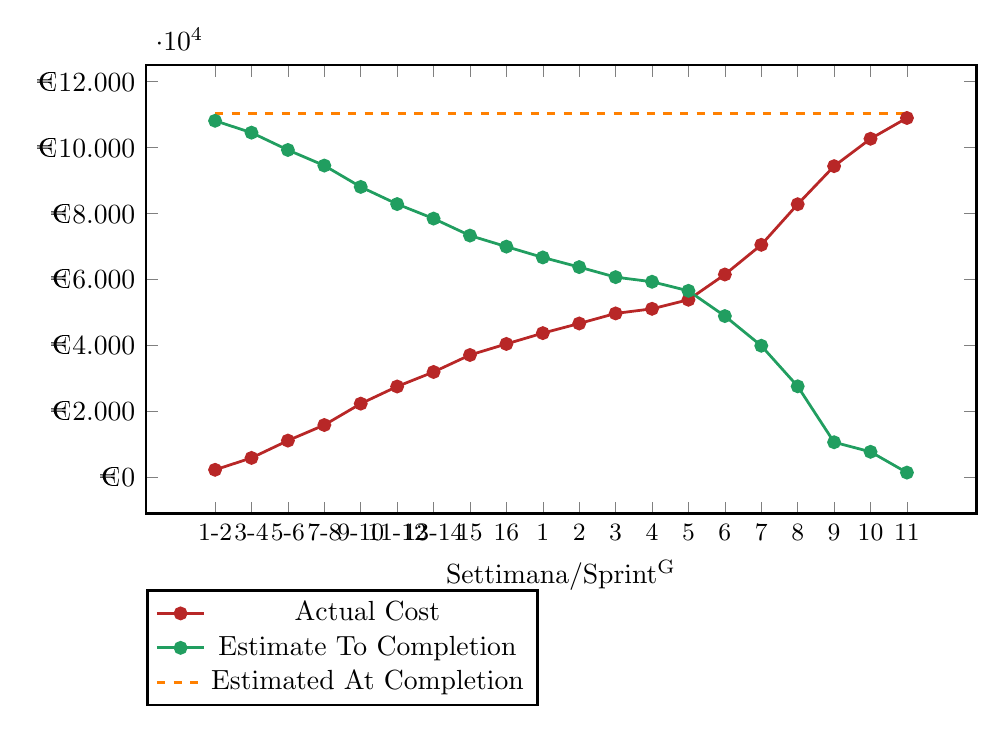
\begin{tikzpicture}
		\begin{axis}[
				xticklabels={1-2, 3-4, 5-6, 7-8, 9-10, 11-12, 13-14, 15, 16, 1, 2, 3, 4, 5, 6,7 ,8,9,10,11},
				xtick={0,1,2,3,...,19},
				xlabel=Settimana/Sprint\textsuperscript{G},
				ytick={0,2000,...,12000},
				x tick label style = {font = \small, text width = 1.6cm, align = center},
				width=\textwidth,
				height=\axisdefaultheight,
				%ylabel=Costo,
				ymax=12500,
				%ymin=-7,
				line width=1.0,
				%yticklabel={\tick\texteuro},
				%y tick label style={xshift=-0.2em,log ticks with fixed point},
				yticklabels={\texteuro0, \texteuro2.000, \texteuro4.000, \texteuro6.000, \texteuro8.000, \texteuro10.000, \texteuro12.000},
				legend columns=1,
				legend style={at={(0.0,-0.3)},anchor=west}				
			]
			]
			\addplot+[sharp plot, red4, mark options={fill=red4}] coordinates { 
				(0,230) (1,590) (2,1115) (3,1587.5) (4,2235) (5,2755) (6,3195) (7,3710) (8,4045) (9,4372.5) (10,4665) (11,4970) 
				(12,5110) (13,5385) (14,6150) (15,7050) (16,8280) (17,9435) (18,10265) (19,10895)
			 };
			\addlegendentry{Actual Cost}
			
			\addplot+[sharp plot, teal6,mark=*,mark options={fill=teal6}] coordinates {
				(0,10810) (1,10450) (2,9925) (3,9452.5) (4,8805) (5,8285) (6,7845)
				(7,7330) (8,6995) (9,6667.5) (10,6375) (11,6070) (12,5930) (13,5655) (14,4890) (15,3990) (16,2760) (17,1065) (18,775) (19,145)
			 };
			\addlegendentry{Estimate To Completion}
			
			\addplot[mark=none, dashed, orange ]  coordinates { (0,11040) (19,11040) };
			\addlegendentry{Estimated At Completion}
			
		\end{axis}
	\end{tikzpicture}
\end{figure}

	\paragraph{RTB\textsuperscript{G}} Il grafico mostra le metriche \textit{Actual Cost} (MPC\textsuperscript{G}-AC)  ossia il costo sostenuto nel periodo evidenziato, \textit{Estimate to Completion} (MPC-EC) ossia il costo rimanente previsto ed infine \textit{Estimated at Completion} ossia il costo totale previsto. 
	Si nota come all'inizio la suddivisione dei periodi era di due settimane fino alla settimana 15 il periodo di sviluppo è stato portato a una settimana questo ha portato ad un aumento del lavoro prodotto. 
	Il periodo RTB\textsuperscript{G} è durato dalla settimana 1 allo sprint\textsuperscript{G} 3.
	
	\paragraph{PB\textsuperscript{G}} Dallo sprint\textsuperscript{G} 5, successivo all'inizio del periodo PB\textsuperscript{G} (sprint 4), si nota un aumento dell'attività del progetto questo è attribuibile all'applicazione dei \textit{feedback} ricevuti dall'esito della fase RTB\textsuperscript{G} e dall'aumento della disponibilità dei componenti dopo la sessione di esami invernale.
	
	\subsubsection{MPC-PV e MPC-EV (\textit{Planned Value} e \textit{Earned Value})}
	
	\begin{figure}[H]
		\captionsetup{textformat=empty,labelformat=blank}
		\caption {MPC-PV e MPC-EV (\textit{Planned Value} e \textit{Earned Value})}
		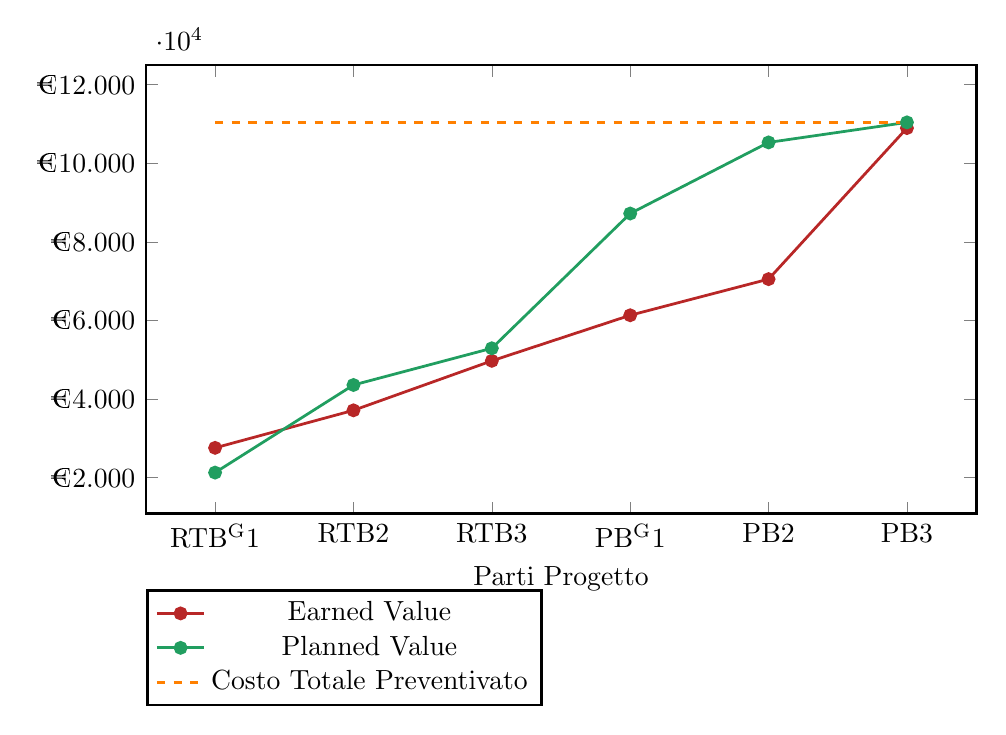
\begin{tikzpicture}
		\begin{axis}[
			xticklabels={RTB\textsuperscript{G}1, RTB2, RTB3,PB\textsuperscript{G}1,PB2,PB3},
			xtick={0,1,2,3,4,5},
			xlabel=Parti Progetto,
			ytick={0,2000,...,12000},
			width=\textwidth,
			height=\axisdefaultheight,
			%ylabel=Costo,
			ymax=12500,
			%ymin=-7,
			line width=1.0,
			%yticklabel={\tick\texteuro},
			%y tick label style={xshift=-0.2em,log ticks with fixed point},
			yticklabels={\texteuro0, \texteuro2.000, \texteuro4.000, \texteuro6.000, \texteuro8.000, \texteuro10.000, \texteuro12.000},
			legend columns=1,
			legend style={at={(0.0,-0.3)},anchor=west}				
			]
			]
			\addplot+[sharp plot, red4, mark options={fill=red4}] coordinates { 
				(0,2755) (1,3710) (2,4970) (3,6130) (4,7050)  (5,10895)
			};
			\addlegendentry{Earned Value}
			
			
			
			
			
			\addplot+[sharp plot, teal6,mark=*,mark options={fill=teal6}] coordinates {
				(0,2125) (1,4355) (2,5290) (3,8720) (4,10530) (5,11040)  
			};
			\addlegendentry{Planned Value}
			
			\addplot[mark=none, dashed, orange ]  coordinates { (0,11040) (5,11040) };
			\addlegendentry{Costo Totale Preventivato}
			
		\end{axis}
	\end{tikzpicture}
\end{figure}
	
	\paragraph{RTB\textsuperscript{G}} Nel primo periodo si nota come il lavoro effettuato sia leggermente maggiore di quello pianificato poi mantenendo lo stesso andamento fino al raggiungimento dei costi pianificati nell'ultimo periodo della fase RTB\textsuperscript{G}.
	
	\paragraph{PB\textsuperscript{G}} Durante il periodo PB\textsuperscript{G} si era pianificato un aumento più rapido nei primi due periodi mentre il gruppo ha mantenuto il trend precedente fino ad un considerevole aumento verso la fine del progetto.
	
		\subsubsection{MPC-CV (\textit{Cost Variance})}
		
\begin{figure}[H]
\captionsetup{textformat=empty,labelformat=blank}
\caption {MPC-CV (Cost Variance)}
	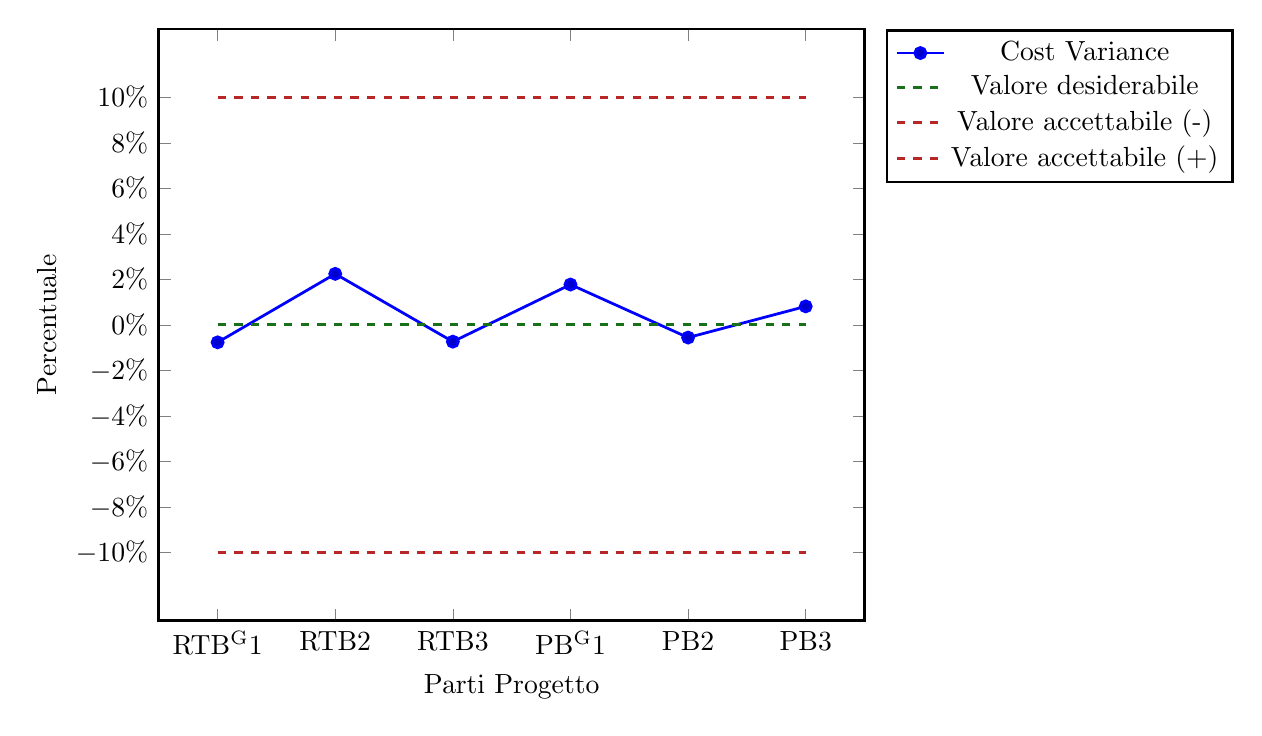
\begin{tikzpicture}
		\begin{axis}[
			xticklabels={RTB\textsuperscript{G}1, RTB2, RTB3,PB\textsuperscript{G}1,PB2,PB3},
			xtick={0,1,2,3,4,5},
			xlabel=Parti Progetto,
			ytick={-10,-8,-6,-4,-2,0,2,4,6,8,10},
			ylabel=Percentuale,
			ymax=13,
			ymin=-13,
			line width=1.0,
			width=300,
			yticklabel={\pgfmathprintnumber{\tick}\%},
			legend style={ 
				legend pos =outer north east
			},
			legend columns=1
			]
			]
			\addplot+[sharp plot, blue] coordinates { (0,-0.77) (1,2.24) (2,-0.74) (3,1.77) (4,-0.56) (5,0.81)};
			\addlegendentry{Cost Variance}
			
			\addplot[mark=none, dashed, green4 ]  coordinates { (0,0) (5,0) };
			\addlegendentry{Valore desiderabile}
			
			\addplot[mark=none, dashed, red4]  coordinates { (0,-10) (5,-10) };
			\addlegendentry{Valore accettabile (-)}
			
			\addplot[mark=none, dashed, red4]  coordinates { (0,10) (5,10) };
			\addlegendentry{Valore accettabile (+)}
			
		\end{axis}
	\end{tikzpicture}
\end{figure}
	
	\paragraph{RTB\textsuperscript{G}} Il grafico rappresenta il rapporto tra i costi sostenuti ed il valore ottenuto mostrato come percentuale.
	Si nota come nella prima fase del periodo il gruppo sia stato leggermente in anticipo sulle aspettative, passando poi in ritardo nel periodo successivo ma concludendo la fase RTB\textsuperscript{G} leggermente in anticipo.
	
	\paragraph{PB\textsuperscript{G}} Dal grafico si deduce un considerevole ritardo nel primo periodo PB\textsuperscript{G} che viene diminuito nel secondo periodo. Alla fine del progetto il valore aumenta leggermente in quanto il gruppo ha terminato non utilizzando tutto il budget a disposizione.\\
	Si noti come in ogni caso il gruppo rispetti i valori di massimo e minimo prestabiliti.
	
	\subsubsection{MPC-SV (\textit{Schedule Variance})}
\begin{figure}[H]
	\captionsetup{textformat=empty,labelformat=blank}
	\caption {MPC-SV (\textit{Schedule Variance})}

	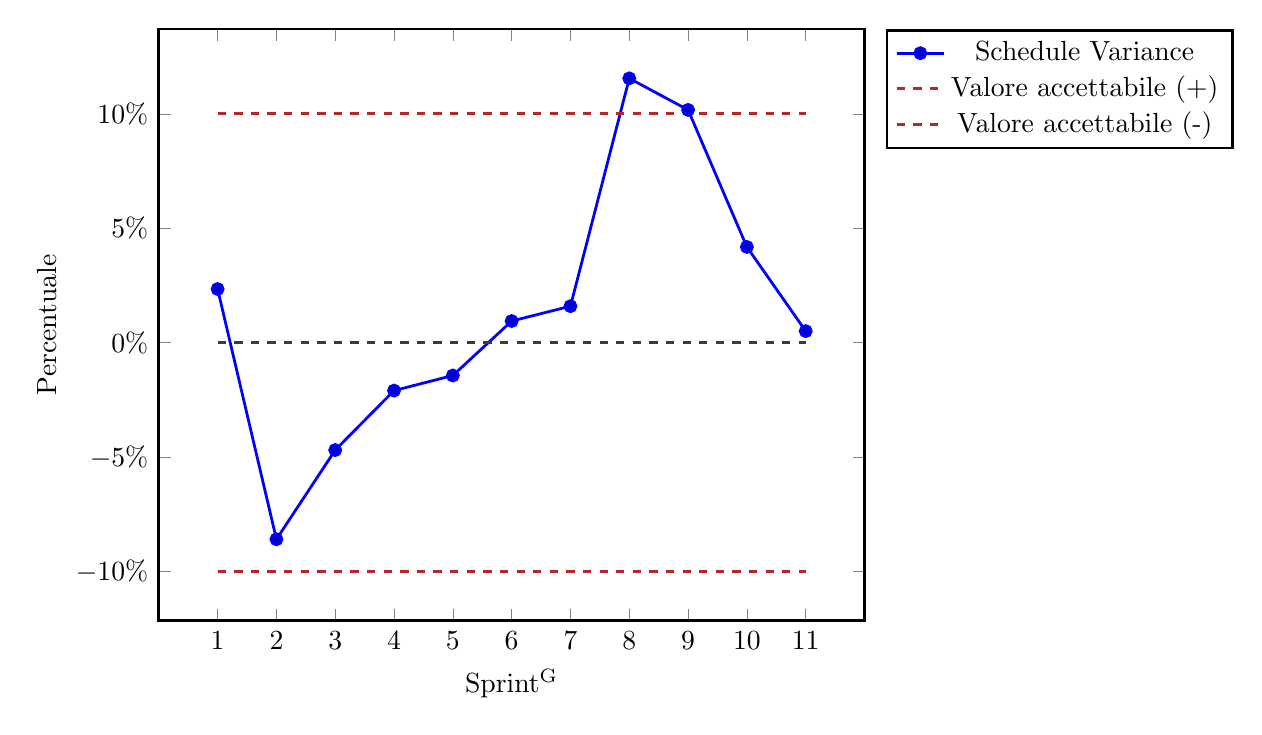
\begin{tikzpicture}
		\begin{axis}[
			xticklabels={1,  2, 3,4,5,6,7,8,9,10,11},
			xtick={0,1,2,3,4,5,6,7,8,9,10},
			xlabel=Sprint\textsuperscript{G},
			ytick={-15,-10,-5,0,5,10,15},
			ylabel=Percentuale,
			line width=1.0,
			width=300,
			yticklabel={\pgfmathprintnumber{\tick}\%},
			legend style={ 
				legend pos =outer north east
			},
			legend columns=1
			]
			]
			\addplot+[sharp plot, blue] coordinates {(0,2.34) (1,-8.6) (2,-4.7) (3,-2.1) (4,-1.44) (5,0.94) (6,1.59) (7,11.55) (8,10.17) (9,4.18) (10,0.5)  };
			\addlegendentry{Schedule Variance}
			
			\addplot[mark=none, dashed, red4 ]  coordinates { (0,10) (10,10) };
			\addlegendentry{Valore accettabile (+)}
			
			\addplot[mark=none, dashed, red4]  coordinates { (0,-10) (10,-10) };
			\addlegendentry{Valore accettabile (-)}
			
			\addplot[mark=none, dashed, gray2]  coordinates { (0,0) (10,0) };
			
		\end{axis}
	\end{tikzpicture}
\end{figure}
	
		\paragraph{RTB\textsuperscript{G}} Il grafico rappresenta il rapporto tra il valore pianificato ed il valore guadagnato. Vengono considerati i periodi finali del periodo RTB\textsuperscript{G} (sprint\textsuperscript{G} 1,2 e 3) ed è evidente che il gruppo era in ritardo sulle aspettative, specialmente nello sprint 2 che viene dimezzato nello sprint 3.
	
	\paragraph{PB\textsuperscript{G}} A partire dallo sprint\textsuperscript{G} 4, inizio del periodo PB\textsuperscript{G}, si nota come il gruppo ha recuperato gran parte del ritardo accumulato e mantiene un aumento costante delle attività fino ad essere in linea con la pianificazione nello sprint 6, il lavoro aumenta considerevolmente nello sprint 7 sforando leggermente il limite superiore ma poi ritornando nei parametri attesi nello sprint finale.
	
	
	\subsubsection{MPC-BV (\textit{Budget Variance})}
	
	\begin{figure}[H]
		\captionsetup{textformat=empty,labelformat=blank}
		\caption {MPC-BV (\textit{Budget Variance})}
		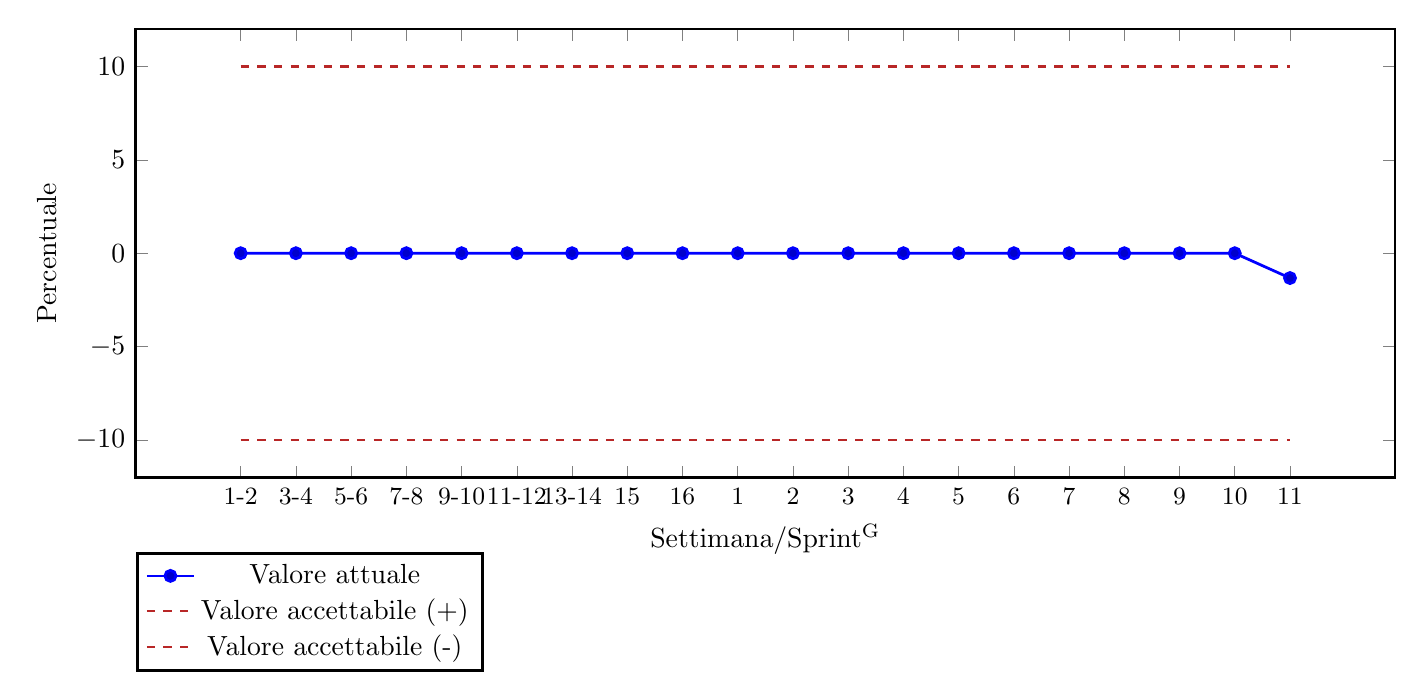
\begin{tikzpicture}
		\begin{axis}[
			xticklabels={1-2, 3-4, 5-6, 7-8, 9-10, 11-12, 13-14, 15, 16, 1, 2, 3, 4, 5, 6,7 ,8, 9 ,10,11},
			xtick={0,1,2,3,...,19},
			xlabel=Settimana/Sprint\textsuperscript{G},
			x tick label style = {font = \small, text width = 1.6cm, align = center},
			width=500,
			height=\axisdefaultheight,
			ylabel=Percentuale,
			ymax=12,
			ymin=-12,
			line width=1.0,			
			legend columns=1,
			legend style={at={(0.0,-0.3)},anchor=west}				
			]
			]
		
			
			\addplot+[sharp plot, blue]  coordinates { (0,0) (1,0) (2,0) (3,0) (4,0) (5,0) (6,0) (7,0) (8,0) (9,0) (10,0) (11,0) (12,0)
			(13,0) (14,0) (15,0) (16,0) (17,0) (18,0) (19,-1.33) };
			\addlegendentry{Valore attuale}
			
			\addplot[mark=none, dashed, red4 ]  coordinates { (0,10) (19,10) };
			\addlegendentry{Valore accettabile (+)}
			
			\addplot[mark=none, dashed, red4]  coordinates { (0,-10) (19,-10) };
			\addlegendentry{Valore accettabile (-)}
			
		\end{axis}
	\end{tikzpicture}
\end{figure}
	
	\paragraph{RTB\textsuperscript{G} e PB\textsuperscript{G}} Si nota dal grafico come il budget per il progetto non sia stato variato durante il proseguimento della fase RTB.
	
	\paragraph{PB\textsuperscript{G}} Alla fine della fae PB il budget è diminuto del 1.33\% (\euro 145,00) in quanto le attività del progetto sono state ritenute concluse.
	
	\subsection{Sviluppo}
	\subsubsection{MPC-RSI (\textit{Requirements Stability Index})}
	
	\pgfplotsset{compat=1.11}
	
\begin{figure}[H]
	\captionsetup{textformat=empty,labelformat=blank}
	\caption {MPC-RSI (\textit{Requirements Stability Index})}
	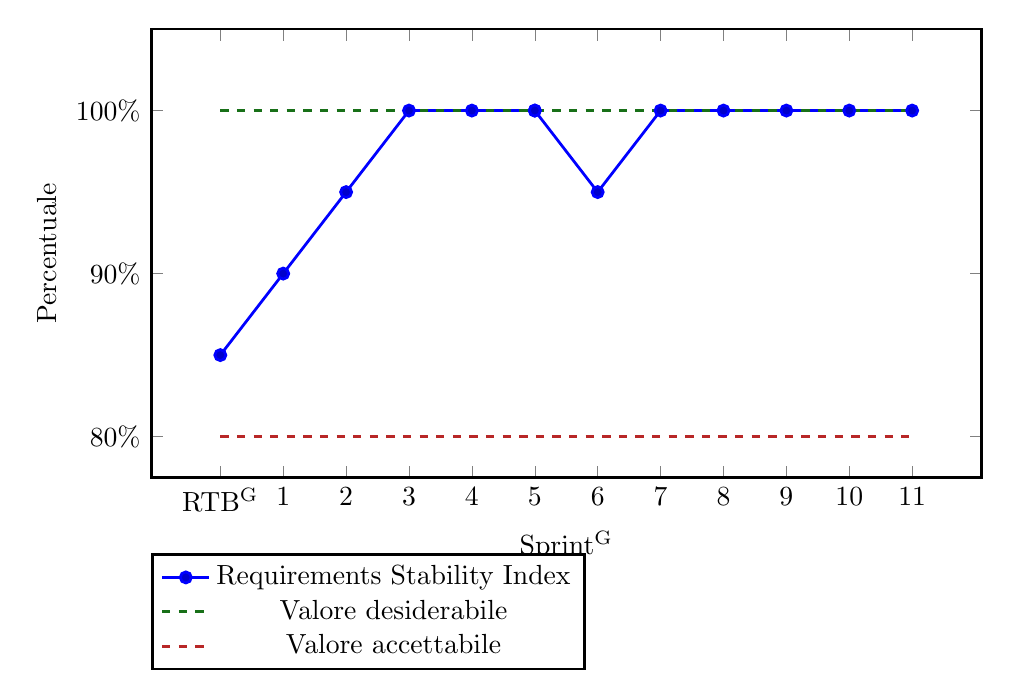
\begin{tikzpicture}
		\begin{axis}[
			xticklabels={RTB\textsuperscript{G}, 1, 2, 3, 4, 5, 6, 7, 8, 9,10,11},
			xtick={0,1,...,11},
			xlabel=Sprint\textsuperscript{G},
			ytick={0,10,...,100},
			ylabel=Percentuale,
			%yticklabels={\pgfmathprintnumber{\tick}\%},
			yticklabel=\pgfmathprintnumber{\tick}\%,
			ymax=105,
			line width=1.0,
			width=\textwidth,
			height=\axisdefaultheight,
			legend columns=1,
			legend style={at={(0.0,-0.3)},anchor=west},
			legend columns=1
			]
			]
			\addplot+[sharp plot, blue] coordinates {(0,85) (1,90) (2,95) (3,100) (4,100) (5,100) (5,100) (6,95) 
				(7,100) (8,100) (9,100) (10,100) (11,100)};
			\addlegendentry{Requirements Stability Index}
			
			\addplot[mark=none, dashed, green4]  coordinates { (0,100) (11,100) };
			\addlegendentry{Valore desiderabile}
			
			\addplot[mark=none, dashed, red4 ]  coordinates { (0,80) (11,80) };
			\addlegendentry{Valore accettabile}
			
		\end{axis}
	\end{tikzpicture}
\end{figure}
	
	\paragraph{RTB\textsuperscript{G}} Il grafico mostra la stabilità dei requisiti nel corso del progetto. Dopo aver ricevuto la correzione del documento di Analisi dei Requisiti\textsuperscript{G} da parte del prof. Cardin si nota un aumento della stabilità dei requisiti, applicando le indicazioni fornite.
	Si è raggiunta la stabilità massima alla fine del periodo RTB\textsuperscript{G} (sprint\textsuperscript{G} 3).
	
	\paragraph{PB\textsuperscript{G}} Il periodo PB\textsuperscript{G} è iniziato con una stabilità del 100\% avendo un calo del 5\% nello sprint\textsuperscript{G} 6 dovuto alla modifica di un requisito\textsuperscript{G} nel documento di Analisi dei Requisti per indicare in maniera più precisa il comportamento del sistema durante il caricamento di una struttura \textit{database}\textsuperscript{G} tramite \textit{file}\textsuperscript{G}.
	
		
	
	\subsubsection{MPC-SOR (\textit{Satisfied Obligatory Requirements})}
	
	\pgfplotsset{compat=1.11}
	
	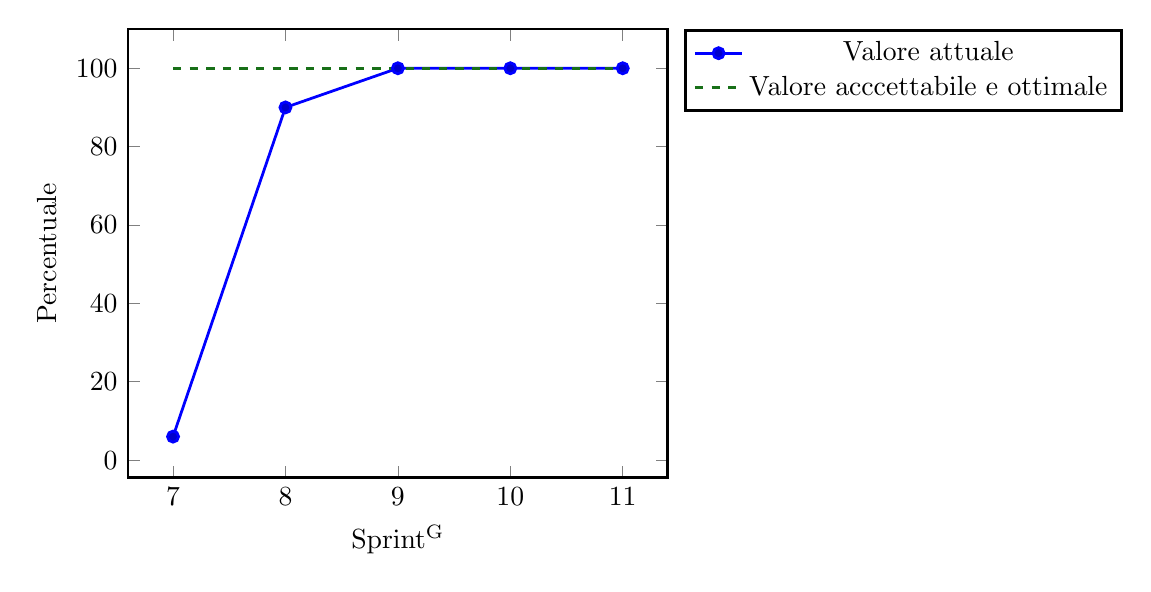
\begin{tikzpicture}
	\begin{axis}[
		xticklabels={7,8,9,10,11},
		xtick={0,1,2,3,4},
		xlabel=Sprint\textsuperscript{G},
		ylabel=Percentuale,
		ymax=110,
		line width=1.0,
		legend style={ 
			legend pos =outer north east
		},
		legend columns=1
		]
		]
		
		\addplot+[sharp plot, blue] coordinates {(0,6) (1,90) (2,100) (3,100) (4,100)};
		\addlegendentry{Valore attuale}
		
		\addplot[mark=none, dashed, green4]  coordinates { (0,100) (4,100) };
		\addlegendentry{Valore acccettabile e ottimale}

		
	\end{axis}
\end{tikzpicture}
		
	\paragraph{PB\textsuperscript{G}} Il grafico mostra la percentuale di requisiti obbligatori soddisfatti. Si nota come nel primo sprint\textsuperscript{G} di sviluppo (sprint 7)  i requisiti\textsuperscript{G} obbligatori non siano stati soddisfatti, questa percentuale cresce al 90\%  nello sprint 8 per poi diventare 100\% negli sprint successivi.
	


\subsection{Gestione di qualità}
	
	\subsubsection{MPC-QMS (\textit{Quality Metrics Satisfied})}
	
	\begin{figure}[H]
		\captionsetup{textformat=empty,labelformat=blank}
		\caption {MPC-CV (Cost Variance)}
		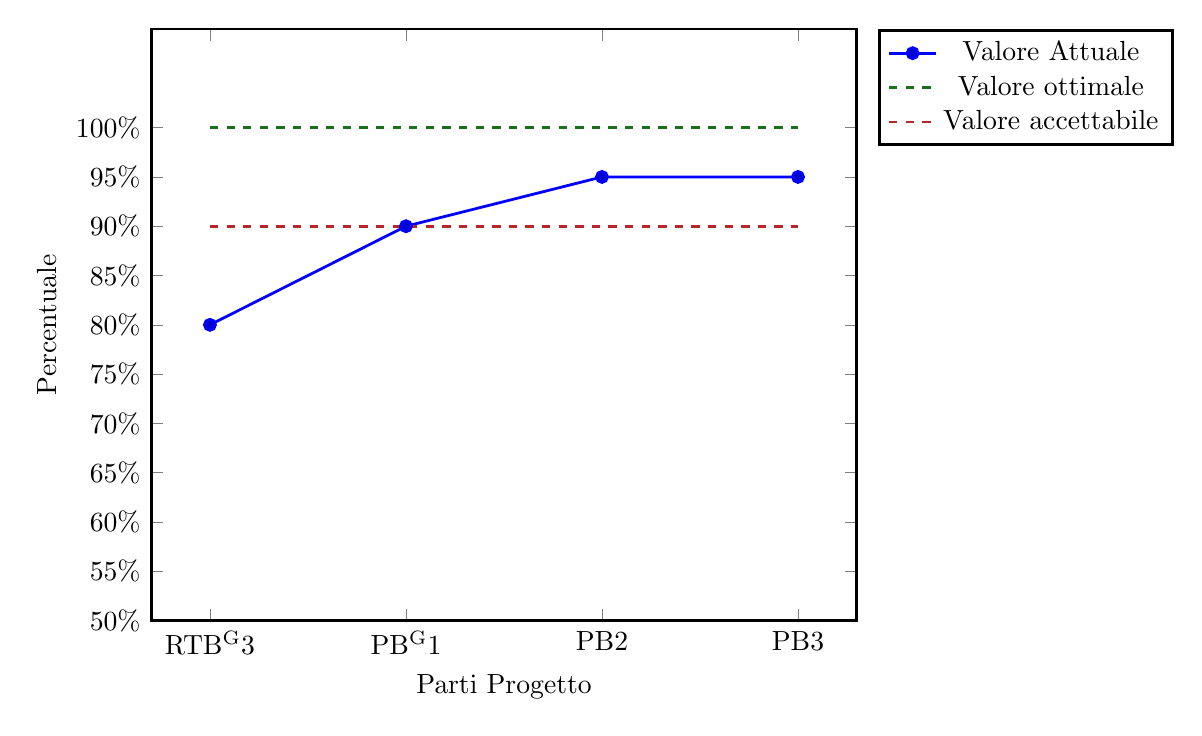
\begin{tikzpicture}
			\begin{axis}[
				xticklabels={RTB\textsuperscript{G}3,PB\textsuperscript{G}1,PB2,PB3},
				xtick={0,1,...,3},
				xlabel=Parti Progetto,
				ytick={0,5,...,100},
				ylabel=Percentuale,
				ymax=110,
				ymin=50,
				line width=1.0,
				width=300,
				yticklabel={\pgfmathprintnumber{\tick}\%},
				legend style={ 
					legend pos =outer north east
				},
				legend columns=1
				]
				]
				\addplot+[sharp plot, blue] coordinates { (0,80) (1,90) (2,95) (3,95) };
				\addlegendentry{Valore Attuale}
				
				\addplot[mark=none, dashed, green4 ]  coordinates { (0,100) (3,100) };
				\addlegendentry{Valore ottimale}
				
				\addplot[mark=none, dashed, red4 ]  coordinates { (0,90) (3,90) };
				\addlegendentry{Valore accettabile}

				
			\end{axis}
		\end{tikzpicture}
	\end{figure}
	
	\paragraph{RTB\textsuperscript{G}} Il grafico rappresenta la percentuale di metriche di qualità soddisfatte nei periodi di progetto.
	Il periodo RTB3 rappresenta il periodo dove è stata ricevuta la valutazione della parte RTB del progetto, si nota che le metriche di qualità non sono state rispettate a sufficienza.
	
	
	\paragraph{PB\textsuperscript{G}} Dal grafico si deduce che c'è stato un aumento delle metriche di qualità soddisfatte fino a raggiungere il 95\%. Non si è raggiunto il 100\% in quanto alcune metriche non sono state soddisfatte (per esempio Schedule Variance).

	
\subsection{Verifica}

\subsubsection{MPC-CC (\textit{Code Coverage})}

\begin{figure}[H]
	\captionsetup{textformat=empty,labelformat=blank}
	\caption {MPC-CC (\textit{Code Coverage)}}

	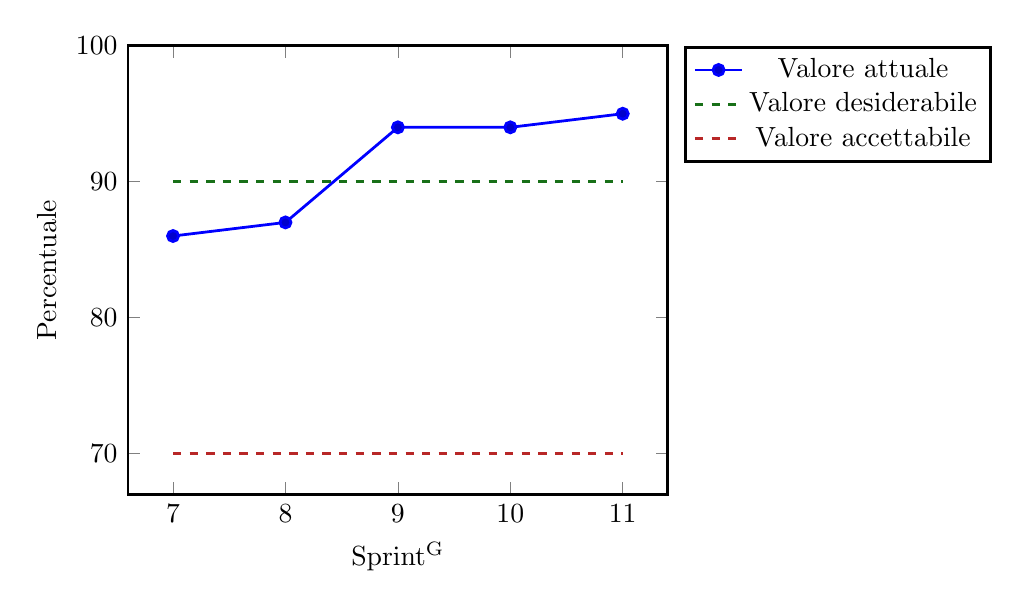
\begin{tikzpicture}
		\begin{axis}[
			xticklabels={7,8,9,10,11},
			xtick={0,1,2,3,4},
			xlabel=Sprint\textsuperscript{G},
			ylabel=Percentuale,
			ymax=100,
			line width=1.0,
			legend style={ 
				legend pos =outer north east
			},
			legend columns=1
			]
			]
			
			\addplot+[sharp plot, blue] coordinates {(0,86) (1,87) (2,94) (3,94) (4,95) };
		\addlegendentry{Valore attuale}
			
			\addplot[mark=none, dashed, green4]  coordinates { (0,90) (4,90) };
			\addlegendentry{Valore desiderabile}
			
			\addplot[mark=none, dashed, red4 ]  coordinates { (0,70) (4,70) };
			\addlegendentry{Valore accettabile}
			
		\end{axis}
	\end{tikzpicture}
	
\end{figure}
	
	\paragraph{RTB\textsuperscript{G}} Il grafico mostra le righe di codice coperte da operazioni di test. 
	Non sono state effettuate operazioni di codifica del prodotto finale nella fase RTB\textsuperscript{G}.
	
	\paragraph{PB\textsuperscript{G}} All'inizio dello sviluppo del prodotto finale si è ottenuto una copertura del 86\% delle linee di codice scritte passando poi al 87\% nel periodo successivo. Dallo sprint 9 si è raggiunta una copertura del 94\%, diventato poi 95\% nel periodo successivo, superando il valore desiderabile di 90\%.\\
	Ad ogni aggiunta del programma viene associato un aumento della copertura del codice alla fine del periodo di sviluppo.

	\subsubsection{MPC-PTP (\textit{Passed Tests Percentage)}}

\begin{figure}[H]
	\captionsetup{textformat=empty,labelformat=blank}
	\caption {MPC-PTP (\textit{Passed Tests Percentage)}}

	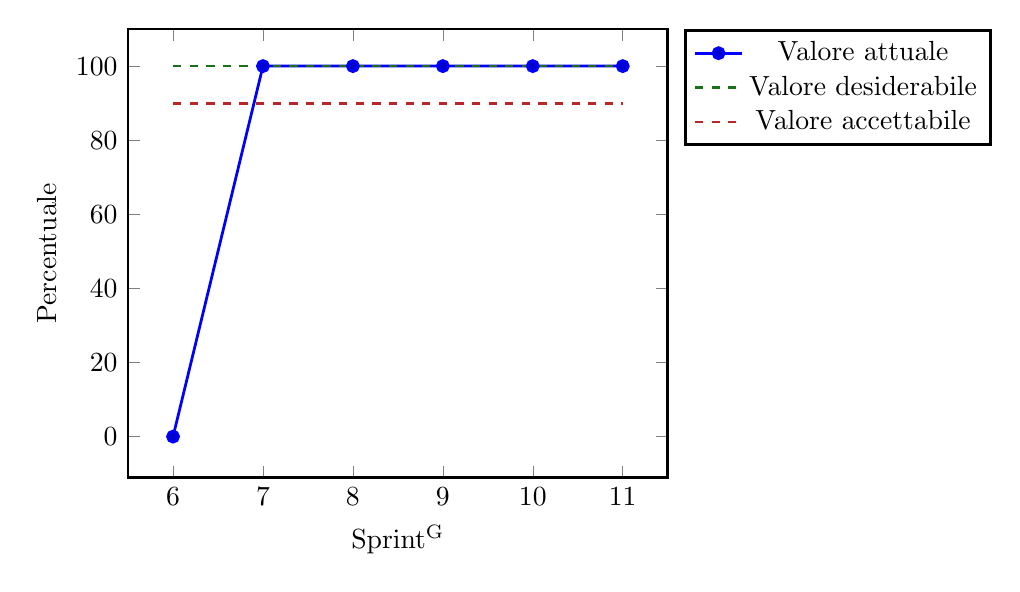
\begin{tikzpicture}
		\begin{axis}[
			xticklabels={6,7,8,9,10,11},
			xtick={0,1,2,3,4,5},
			xlabel=Sprint\textsuperscript{G},
			ylabel=Percentuale,
			ymax=110,
			line width=1.0,
			legend style={ 
				legend pos =outer north east
			},
			legend columns=1
			]
			]
			
			\addplot+[sharp plot, blue] coordinates {(0,0) (1,100) (2,100) (3,100) (4,100) (5,100) };
			\addlegendentry{Valore attuale}
			
			\addplot[mark=none, dashed, green4]  coordinates { (0,100) (5,100) };
			\addlegendentry{Valore desiderabile}
			
			\addplot[mark=none, dashed, red4 ]  coordinates { (0,90) (5,90) };
			\addlegendentry{Valore accettabile}
			
		\end{axis}
	\end{tikzpicture}
\end{figure}
	
	\paragraph{RTB\textsuperscript{G}} Il grafico mostra la percentuale di test con esito positivo.
	Non sono state effettuate operazioni di codifica del prodotto finale nella fase RTB\textsuperscript{G}.
	
	\paragraph{PB\textsuperscript{G}} Si nota come ogni test codificato abbia esito positivo, questo avviene perché ogni modifica apportata al prodotto viene accompagnata da test che la verificano con successo.
	
	\subsection{Processi organizzativi}
	
	\subsubsection{MPC-NCR (\textit{Non-Calculated Risks)}}
	
\begin{figure}[H]
	\captionsetup{textformat=empty,labelformat=blank}
	\caption {MPC-NCR (\textit{Non-Calculated Risks)}}
	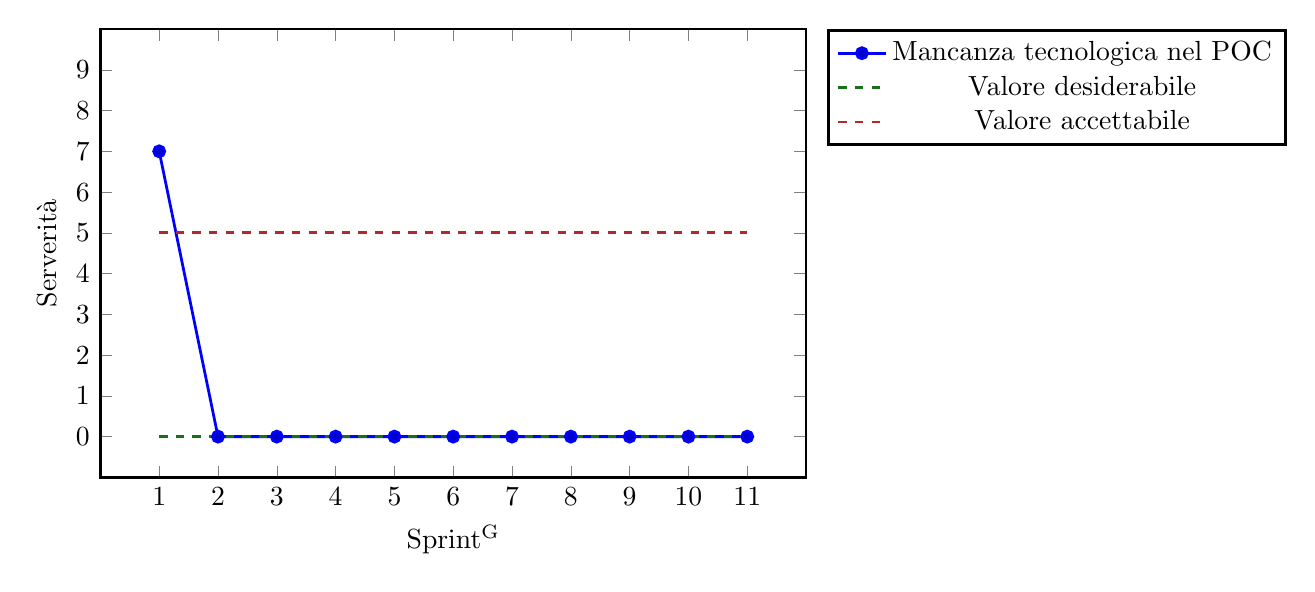
\begin{tikzpicture}
		\begin{axis}[
			xticklabels={ 1,  2,...,11},
			xtick={0,1,...,10},
			xlabel=Sprint\textsuperscript{G},
			ytick={0,1,...,9},
			ylabel=Serverità,
			yticklabels={0,1,...,9},
			ymax=10,
			line width=1.0,
			width=300,
			height=\axisdefaultheight,
			legend style={ 
				legend pos =outer north east
			},
			legend columns=1
			]
			]
			\addplot+[sharp plot, blue] coordinates {(0,7) (1,0) (2,0) (3,0) (4,0) (5,0) (6,0) (7,0) (8,0) (9,0) (10,0) };
			\addlegendentry{Mancanza tecnologica nel POC}
			
			\addplot[mark=none, dashed, green4]  coordinates { (0,0) (10,0) };
			\addlegendentry{Valore desiderabile}
			
			\addplot[mark=none, dashed, red4 ]  coordinates { (0,5) (10,5) };
			\addlegendentry{Valore accettabile}
			
		\end{axis}
	\end{tikzpicture}
\end{figure}
	
	\paragraph{RTB\textsuperscript{G}} Il grafico mostra i rischi non pianificati sostenuti nel corso del progetto e la loro gravità.
	Si nota un rischio considerevole nel primo sprint\textsuperscript{G}, questo era dato da una mancanza tecnologica presente nel POC\textsuperscript{G} presentato al prof. Cardin, questo rischio è stato colmato aumentando le funzionalità del POC e utilizzando le tecnologie non utilizzate in precedenza.
	
	\paragraph{PB\textsuperscript{G}} Non sono stati sostenuti rischi non pianificati nel periodo PB\textsuperscript{G}.
	
	
	\subsection{Documenti}
	
	\subsubsection{MPD-IG (Indice Gulpease)}
	
\begin{figure}[H]
	\captionsetup{textformat=empty,labelformat=blank}
	\caption {MPD-IG (Indice Gulpease)}
	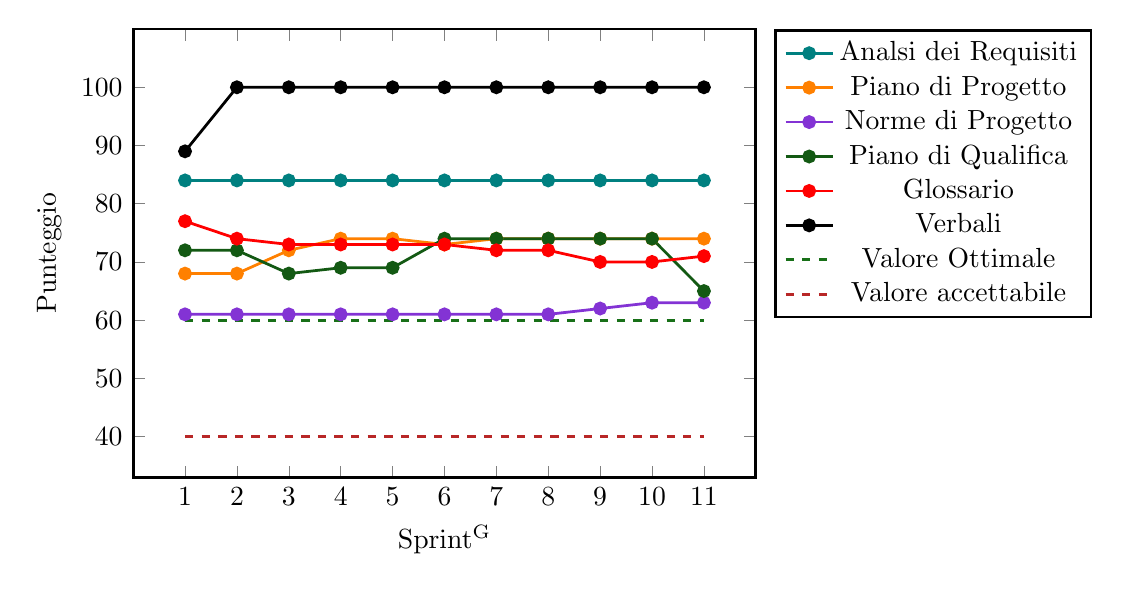
\begin{tikzpicture}
		\begin{axis}[
			xticklabels={ 1,2,...,11},
			xtick={0,1,...,10},
			xlabel=Sprint\textsuperscript{G},
			ytick={30,40,50,60,70,80,90,100},
			ylabel=Punteggio,
			ymax=110,
			line width=1.0,
			width=270,
			height=\axisdefaultheight,
			legend style={ 
				legend pos =outer north east
			},
			legend columns=1
			]
			]
			\addplot+[sharp plot, teal, mark=*, solid, mark options={fill=teal}] coordinates {(0,84) (1,84) (2,84) (3,84) (4,84) (5,84)  (6,84)  (7,84) (8,84) (9,84) (10,84) };
			\addlegendentry{Analsi dei Requisiti}
			
			\addplot+[sharp plot, orange, solid, mark=*, mark color=orange, mark options={fill=orange}] coordinates {(0,68) (1,68) (2,72) (3,74)
			(4,74) (5,73) (6,74) (7,74) (8,74) (9,74) (10,74) };
			\addlegendentry{Piano di Progetto}
			
			\addplot+[sharp plot,violet4, solid, mark=*, mark options={fill=violet4}] coordinates {(0,61) (1,61) (2,61) (3,61) (4,61) (5,61) (6,61) 
			(7,61) (8,62) (9,63) (10,63) };
			\addlegendentry{Norme di Progetto}
			
			\addplot+[sharp plot,green3, solid, mark=*, mark options={fill=green3}] coordinates {(0,72) (1,72) (2,68) (3,69) (4,69) (5,74) 
				(6,74) (7,74) (8,74) (9,74) (10,65) };
			\addlegendentry{Piano di Qualifica}
			
			\addplot+[sharp plot, red, solid, mark=*, mark options={fill=red}] coordinates {(0,77) (1,74) (2,73) (3,73) (4,73) (5,73)
			(6,72) (7,72) (8,70) (9,70) (10,71) };
			\addlegendentry{Glossario}			
			
			\addplot+[sharp plot, black, solid, mark=*, mark options={fill=black}] coordinates {(0,89) (1,100) (2,100) (3,100) (4,100)
			(5,100) (6,100) (7,100) (8,100) (9,100) (10,100) };
			\addlegendentry{Verbali}			
			
			\addplot[mark=none, dashed, green4, mark=none]  coordinates { (0,60) (10,60) };
			\addlegendentry{Valore Ottimale}
			
			\addplot[mark=none, dashed, red4,mark=none]  coordinates { (0,40) (10,40) };
			\addlegendentry{Valore accettabile}
			
		\end{axis}
	\end{tikzpicture}
\end{figure}
	
	\paragraph{RTB\textsuperscript{G}} Il grafico mostra il punteggio raggiunto dai vari documenti per quanto riguarda l'indice di leggibilità Gulpease. Si è scelto il valore 60 come limite minimo, questo rappresenta un livello di comprensione di una persona con un diploma di scuola media.\\
	Si noti come i documenti mantengano un valore ampiamente sufficiente ad eccezione del documento di Norme di Progetto\textsuperscript{G} che comunque mantiene il valore minimo accettabile. Si noti inoltre come la leggibilità dei verbali aumenti di 10 punti nelle ultime fasi del periodo RTB\textsuperscript{G}.
	
	\paragraph{PB\textsuperscript{G}} La maggior parte dei documenti mantiene lo stesso punteggio, le differenze si notano nei documenti: 
	\begin{itemize}
		\item Piano di Qualifica\textsuperscript{G}: Aumenta di complessità negli sprint\textsuperscript{G} 3,4 e 5, successivamente aumenta il suo punteggio dallo sprint 6 e aumentando la sua complessità e diminuendo il punteggio nello sprint 11.
		\item Glossario\textsuperscript{G}: Si nota come aumentando le definizioni dei termini presenti nel documento aumenti la sua complessità;
		\item Norme di Progetto\textsuperscript{G}: Si nota un leggero aumento del punteggio nello sprint\textsuperscript{G} 9;
	\end{itemize}
	
	\subsubsection{MPD-CO (Correttezza Ortografica)}
	
\begin{figure}[H]
	\captionsetup{textformat=empty,labelformat=blank}
	\caption {MPD-CO (Correttezza Ortografica)}
	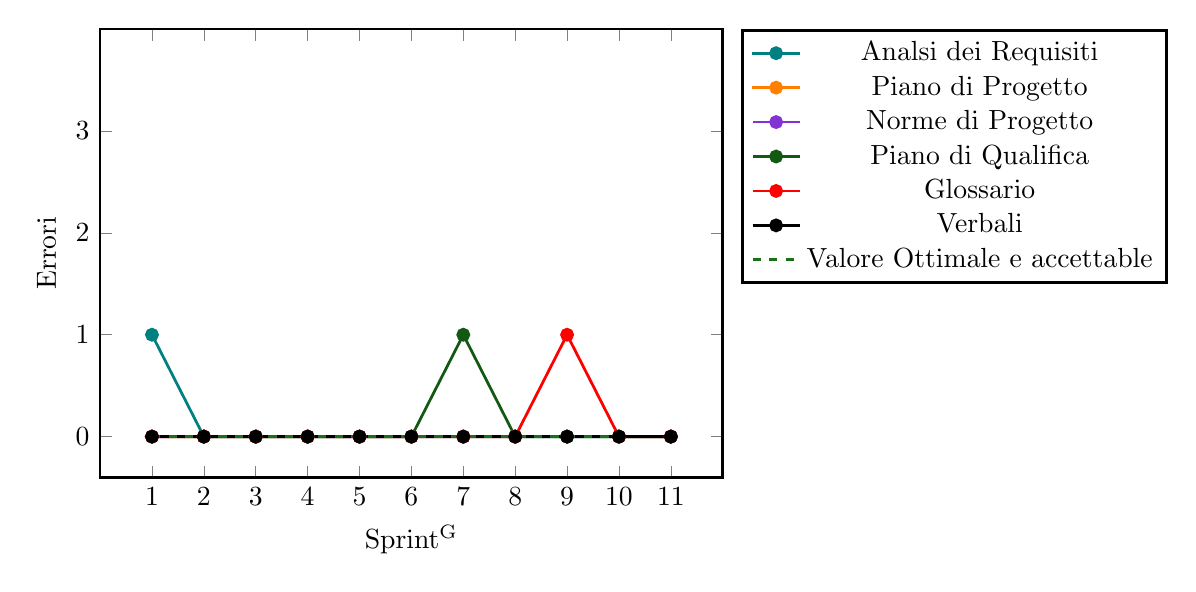
\begin{tikzpicture}
		\begin{axis}[
			xticklabels={ 1,  2,  3,...,11},
			xtick={0,1,2,...,10},
			xlabel=Sprint\textsuperscript{G},
			ytick={0,1,2,3},
			ylabel=Errori,
			ymax=4,
			line width=1.0,
			width=270,
			height=\axisdefaultheight,
			legend style={ 
				legend pos =outer north east
			},
			legend columns=1
			]
			]
			\addplot+[sharp plot, teal, mark=*, solid, mark options={fill=teal}] coordinates {(0,1) (1,0) (2,0) (3,0) (4,0) (5,0) (6,0) (7,0) (8,0) (9,0) (10,0) };
			\addlegendentry{Analsi dei Requisiti}
			
			\addplot+[sharp plot, orange, solid, mark=*, mark color=orange, mark options={fill=orange}] coordinates {(0,0) (1,0) (2,0) 
			(3,0) (4,0) (5,0) (6,0) (7,0) (8,0) (9,0) (10,0) };
			\addlegendentry{Piano di Progetto}
			
			\addplot+[sharp plot,violet4, solid, mark=*, mark options={fill=violet4}] coordinates {(0,0) (1,0) (2,0) (3,0) (4,0) (5,0) (6,0) (7,0) (8,0) (9,0) (10,0)};
			\addlegendentry{Norme di Progetto}
			
			\addplot+[sharp plot,green3, solid, mark=*, mark options={fill=green3}] coordinates {(0,0) (1,0) (2,0) (3,0) (4,0) (5,0) (6,1) (7,0) (8,0) (9,0) (10,0) };
			\addlegendentry{Piano di Qualifica}
			
			\addplot+[sharp plot, red, solid, mark=*, mark options={fill=red}] coordinates {(0,0) (1,0) (2,0) (3,0) (4,0) (5,0) (6,0) (7,0) (8,1) (9,0) (10,0)};
			\addlegendentry{Glossario}			
			
			\addplot+[sharp plot, black, solid, mark=*, mark options={fill=black}] coordinates {(0,0) (1,0) (2,0) (3,0) (4,0) (5,0) (6,0) (7,0) (8,0) (9,0) (10,0)  };
			\addlegendentry{Verbali}			
			
			\addplot[mark=none, dashed, green4, mark=none]  coordinates { (0,0) (9,0) };
			\addlegendentry{Valore Ottimale e accettable}
		
		\end{axis}
	\end{tikzpicture}
\end{figure}
	
	\paragraph{RTB\textsuperscript{G}} Il grafico mostra gli errori ortografici nei documenti nelle fasi finali del periodo RTB\textsuperscript{G}. Sono stati presenti alcuni errori ma grazie al controllo ortografico dei programmi utilizzati nella redazione dei documenti questi sono stati limitati.
	
	\paragraph{PB\textsuperscript{G}} Gli errori presenti nel periodo PB sono stati corretti come nel periodo RTB.
	
	\subsection{Software}
	
	\subsubsection{MPD-CR (Copertura dei Requisiti)}
	\pgfplotsset{compat=1.11}
	
\begin{figure}[H]
	\captionsetup{textformat=empty,labelformat=blank}
	\caption {MPD-CR (Copertura dei Requisiti)}
	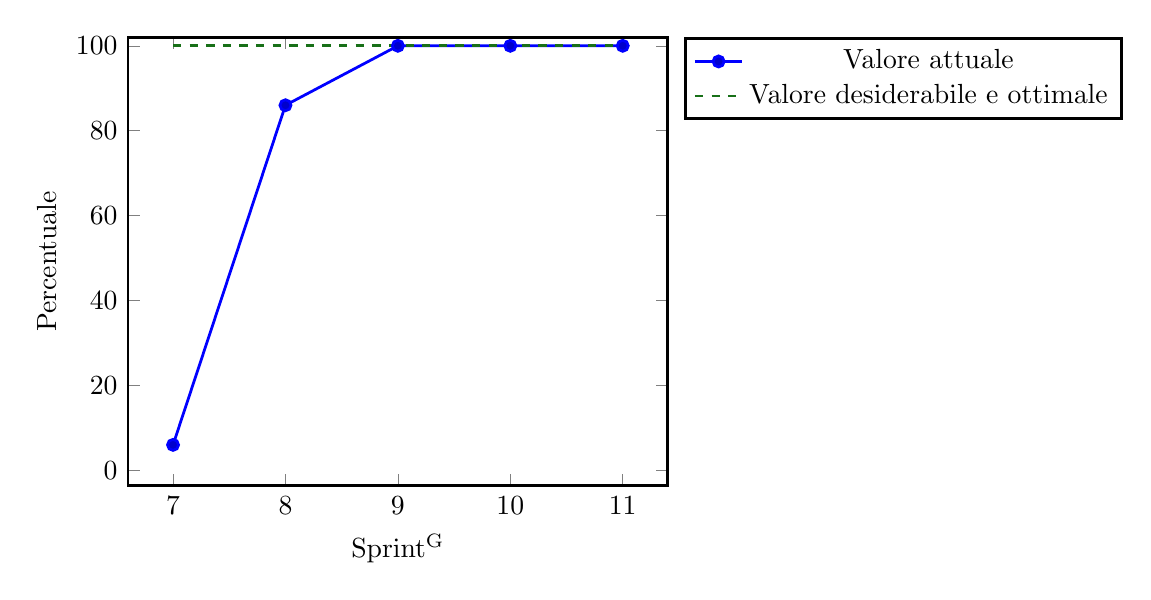
\begin{tikzpicture}
		\begin{axis}[
			xticklabels={7,8,9,10,11},
			xtick={0,1,2,3,4},
			xlabel=Sprint\textsuperscript{G},
			ylabel=Percentuale,
			ymax=102,
			line width=1.0,
			legend style={ 
				legend pos =outer north east
			},
			legend columns=1
			]
			]
						
			\addplot+[sharp plot, blue] coordinates {(0,6) (1,86) (2,100) (3,100) (4,100) };
			\addlegendentry{Valore attuale}
			
			\addplot[mark=none, dashed, green4]  coordinates { (0,100) (4,100) };
			\addlegendentry{Valore desiderabile e ottimale}
			
	
			
		\end{axis}
	\end{tikzpicture}
\end{figure}
	
	\paragraph{PB\textsuperscript{G}} Il grafico mostra la percentuale di copertura dei requisiti espressi nel documento di Analisi dei Requisti durante la realizzazione del prodotto \textit{software}\textsuperscript{G}.\\
	All'inizio della codifica sono stati coperti il 6\% dei requisiti per poi passare al 86\% nel periodo successivo, è stata raggiunta la massima copertura nello sprint\textsuperscript{G} 9.
	
	\subsubsection{MPD-CD (\textit{Code Duplication})}
	
		\begin{longtblr}[
		caption = {MPC-CD (Code Duplication)},
		]
		{
			colspec={|Q[0.15\linewidth]|Q[0.15\linewidth]|Q[0.15\linewidth]|},
			columns={halign=c},
			row{1}={halign=c},
			row{odd} = {gray!20},
			row{1}={teal!50},
			%caption=Tabella 1
		}
		\hline
		\textbf{Valore Accettabile} & \textbf{Valore Ottimale} & \textbf{Valore Ottenuto}\\
		\hline
		0 & 0 & 0\\
		\hline
		
	\end{longtblr}
	
	\paragraph{PB\textsuperscript{G}} La tabella mostra il numero accettabile, ottimale e ottenuto di righe di codice duplicato. Questo valore indica la manutenibilità del \textit{software}\textsuperscript{G} prodotto riducendo la difficoltà di apportare modifiche in futuro.
	
	\subsubsection{MPD-CS (\textit{Code Smell})}
	
			\begin{longtblr}[
			caption = {MPD-CS - ()Code Smell)},
			]
		{
			colspec={|Q[0.15\linewidth]|Q[0.15\linewidth]|Q[0.15\linewidth]|},
			columns={halign=c},
			row{1}={halign=c},
			row{odd} = {gray!20},
			row{1}={teal!50},
			%caption=Tabella 1
		}
		\hline
		\textbf{Valore Accettabile} & \textbf{Valore Ottimale} & \textbf{Valore Ottenuto}\\
		\hline
		$<$ 3 & 0 & 0\\
		\hline
		
	\end{longtblr}
	
	\paragraph{PB\textsuperscript{G}} La tabella mostra il numero accettabile, ottimale e ottenuto di \textit{Code Smell} (letteralmente Codice Odoroso) ossia di problemi di progettazione o di struttura del codice. Il valore ottenuto indica che eventuali problemi sono stati risolti, per individuare questo problemi si è utilizzato il \textit{software}\textsuperscript{G} SonarQube.
	
	
	\subsubsection{MPD-BS (Browser Supportati)}
	\pgfplotsset{compat=1.11}
	
\begin{figure}[H]
	\captionsetup{textformat=empty,labelformat=blank}
	\caption {MPD-BS (Browser Supportati)}
	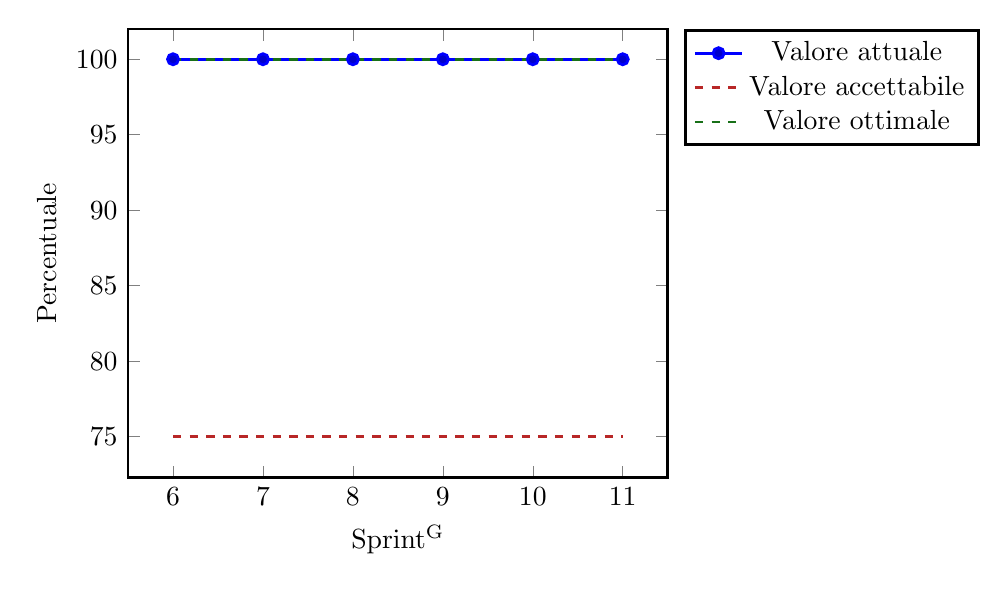
\begin{tikzpicture}
		\begin{axis}[
			xticklabels={6,7,...,11},
			xtick={0,1,...,5},
			xlabel=Sprint\textsuperscript{G},
			ylabel=Percentuale,
			ymax=102,
			line width=1.0,
			legend style={ 
				legend pos =outer north east
			},
			legend columns=1
			]
			]
			
			\addplot+[sharp plot, blue] coordinates {(0,100) (1,100) (2,100) (3,100) (4,100) (5,100)};
			\addlegendentry{Valore attuale}
			
				\addplot[mark=none, dashed, red4,mark=none]  coordinates { (0,75) (5,75) };
		\addlegendentry{Valore accettabile}
			
			\addplot[mark=none, dashed, green4]  coordinates { (0,100) (5,100) };
			\addlegendentry{Valore ottimale}
			
		\end{axis}
	\end{tikzpicture}
\end{figure}
	
	\paragraph{PB\textsuperscript{G}} Il grafico mostra la percentuale dei \textit{browser}\textsuperscript{G} supportati secondo quelli specificati nel documento di Analisi dei Requisti. 
	Si noti come tutti i \textit{browser} siano stati supportati dall'inizio della codifica, questo perché le tecnologie web utilizzate nel progetto sono ampiamente supportate dai \textit{browser} selezionati.
	
	\section{Valutazioni delle attività di verifica}
	In questa sezione si riportano le valutazioni sulle criticità incontrate nel corso dello svolgimento del progetto e le correzioni applicate ad esse.
	
	\subsection{Organizzazione}
	
	\begin{longtblr}[
	caption = {Valutazioni - Organizzazione},
	]
		{
			colspec={|Q[0.12\linewidth]|Q[0.35\linewidth]|Q[0.08\linewidth]|Q[0.35\linewidth]|},
			rows={halign=l},
			column{1}={halign=c},
			column{3}={halign=c},
			column{4}={halign=c},
			row{1}={halign=c},
			row{odd} = {gray!20},
			row{1}={teal!50},
		}
		\hline
		\textbf{Criticità} & \textbf{Descrizione} & \textbf{Gravità} & \textbf{Soluzione} \\
		\hline
		Suddivisione dei compiti & Utilizzando Trello come sistema di \textit{Issue\textsuperscript{G} Tracking} non era chiaro come suddividere i compiti  & Media & Si è passati a Jira\textsuperscript{G} che permette una netta divisione dei compiti per ruolo e arco temporale \\
		\hline
		Verifica & Nei periodi iniziali del progetto non era chiaro quando effettuare l'attività di verifica & Media & Si è aggiunto uno \textit{step} di verifica da completare prima della terminazione del'attività \\
		\hline
	\end{longtblr}
	
	\subsection{Strumenti utilizzati}
	
	\begin{longtblr}[
	caption = {Valutazioni - Strumenti Utilizzati},
	]
		{
			colspec={|Q[0.12\linewidth]|Q[0.35\linewidth]|Q[0.08\linewidth]|Q[0.35\linewidth]|},
			rows={halign=l},
			column{1}={halign=c},
			column{3}={halign=c},
			column{4}={halign=c},
			row{1}={halign=c},
			row{odd} = {gray!20},
			row{1}={teal!50},
		}
		\hline
		\textbf{Criticità} & \textbf{Descrizione} & \textbf{Gravità} & \textbf{Soluzione} \\
		\hline
		Trello & Utile all'inizio del progetto ma non permette la gestione delle attività con \textit{Scrum} & Media & Si è passati a Jira\textsuperscript{G} come \textit{Issue Tracking System} \\
		\hline
		Jira\textsuperscript{G} & Molti componenti del gruppo non conoscevano il programma & Bassa & Sono state consultate le guide a disposizione ed il progetto è stato impostato da chi aveva più familiarità con esso\\
		\hline
		Django\textsuperscript{G} & Alcuni componenti hanno avuto difficoltà ad imparare il \textit{framework}\textsuperscript{G} & Bassa & Le lacune sono state colmate attraverso la documentazione del \textit{software}\textsuperscript{G} e tramite suggerimenti di alcuni componenti. \\
		\hline
		
		
	\end{longtblr}
	
	\subsection{Ruoli}
	
	Al momento non sono stati rilevate criticità per quanto riguarda l'organizzazione dei ruoli. 
	
	
	
\end{document}
